\documentclass[12pt,a4paper]{article}
\usepackage{amsmath}
\usepackage{amsfonts}
\usepackage{amssymb}
\usepackage{amsthm}
\usepackage{enumitem}
\usepackage{setspace}
\usepackage{geometry}
\usepackage{stmaryrd}
\usepackage{graphics}
\usepackage[linesnumbered,vlined,boxruled]{algorithm2e}
\usepackage{algpseudocode}
\usepackage{import}
\usepackage{parskip}
\usepackage{bbm}
\usepackage{natbib}
\usepackage{setspace}
\usepackage[dvipsnames]{xcolor}
\usepackage[citecolor=blue,colorlinks=true,linkcolor=blue]{hyperref}
\setcitestyle{authoryear,round,citesep={;},aysep={,},yysep={;}}
\usepackage{color}
\geometry{
left = 20mm,
right = 20mm
}
\usepackage[utf8]{inputenc}
\usepackage{csquotes}
%\usepackage[english]{babel}
\usepackage{graphicx}
\newtheorem{theorem}{Theorem}[section]
\newtheorem{corollary}{Corollary}[theorem]
\newtheorem{lemma}[theorem]{Lemma}
\newtheorem{proposition}{Proposition}
\usepackage{nccmath}
\geometry{
left = 20mm,
right = 20mm
}
\begin{document}
\section{Piecewise Deterministic Processes}
Piecewise Deterministic Processes (PDPs) are stochastic processes that jump randomly at an almost surely countable number of random times but otherwise evolve deterministically in continuous time. In this chapter, we give an introduction to this class of models and then give a mathematical representation of this class of models.

Let $(\tau_j,\phi_j)_{j \in \mathbb{N}}$ be a stochastic process that represents the random jump times and the corresponding jump values. Moreover, all the $\tau$'s will take values such that $\tau_0 = 0$ and $\tau_0<\tau_1<\tau_2<...$. We also define $\Phi$ to be the support for all the jump values $(\phi_j)_{j \in \mathbb{N}}$. A Piecewise Deterministic Process (PDP) is a continuous time stochastic process $(\zeta_t)_{t \geq 0}$ such that $\zeta_0 := \phi_0$ and 
$$\zeta_t := F^{\theta}(t|\tau_{v_t},\phi_{v_t})$$
where $v_t := \sup \{j \in \mathbb{N}|\tau_j \leq t \}$ represents the latest jump time before time $t$. Hence, a piecewise deterministic process will evolve deterministically according to $F^{\theta}$ after time $\tau_{j}$ until it reaches the next jump time $\tau_{j+1}$. Here, we use $\theta$ to represent all the static parameters used in the model. Suppose that we also have a sequence of known discrete times $0=t_0<t_1<t_2<...$ and define $k_n := v_{t_n}$ to be the number of jumps before time $t_n$  and \(\zeta_{[a,b]} := \left\{\zeta_t| t \in [a,b]\right\}\) be the PDP in the time interval \([a,b]\). It is clear that the process $\zeta_{[0,t_n]}$ can be completely determined by $\left(K_n,\tau_{1:K_n},\phi_{1:K_n},\phi_0\right)$ and the deterministic function \(F^{\theta}\). For simplicity, we propose a Markovian prior on the jump times and jump values in the interval $[0,t_n]$, i.e.
\begin{multline}
\label{eqn:Chap1-PDMP-Prior}
    p_n^{\theta}(k_n,\tau_{1:k_n},\phi_{1:k_n},\phi_0) = S^{\theta}(\tau_{k_n},t_n)q_0^{\theta}(\phi_0)\mathbbm{I}_{(0,t_n]}(\tau_{k_n})\mathbbm{I}(0 < \tau_1 < \tau_2 <.. <\tau_{k_n} < t_n)\\
    \times \prod_{j=1}^{n} f^{\theta}(\tau_j|\tau_{j-1}) g^{\theta}(\phi_j|\tau_j,\tau_{j-1},\phi_{j-1})
\end{multline}
Where \(S^{\theta}(\tau_{k_n},t_n):= 1- \int_{\tau_{k_n}}^{t_n} f^{\theta}(s|\tau_{k_n})\,ds\) denotes the probability that no jump occurring in the interval $(\tau_{k_n},t_n]$ and $f^{\theta}$, $g^{\theta}$ represents the conditional probability density of the jump times and the associated jump values. Note that we also included the density of $k_n$, the number of jumps up to $t_n$ in the posterior $\pi_n$. The reason why we included it in the posterior is that $\pi_n$ can therefore be defined on the increasing subsets of the same space 
\begin{equation*}
    \Tilde{E}_n = \bigcup_{k=0}^{\infty} \left\{\{k\}\times T_{n,k} \times \Phi^{k+1}\right\}
\end{equation*}
where $T_{n,k} := \left\{(\tau_1,...,\tau_k) \in (0,\infty)^k : 0 < \tau_1 <...< \tau_k <= tn\right\}$.The Markovian structure of the process implies that inter-jump times $\tau_n - \tau_{n-1}$ are independent with each other and the jump value $\phi_n$ at $\tau_n$ will only depend on the previous jump value $\phi_{n-1}$ and the latest inter-jump time $\tau_n - \tau_{n-1}$.

In the real settings, such a continuous time stochastic process can only be observed at discrete times with some measurement errors. Let $y_{(s,t]}$ be the observations obtained in the interval $(s,t]$ and $p^{\theta}(y_{(s,t]}|\zeta_{(s,t]})$ be the density of the observations given the PDP. We also assume that the observations obtained in disjoint intervals are conditionally independent given the PDP. Hence, we will have that 

\begin{equation}
\label{eqn:Chap1-PDMP-Likelihood}
    p^{\theta}(y_{(0,t_n]}|\zeta_{(0,t_n]}) = p^{\theta}(y_{(\tau_{k_n},t_n]}|\tau_{k_n},\phi_{k_n}) \prod_{j=1}^{k_n} p^{\theta}(y_{(\tau_{j-1},\tau_j]}|\tau_{j-1},\phi_{j-1})
\end{equation}


The posterior density of the jump times and values up to $t_n$ will then be given by 
\begin{equation}
\label{eqn:Chap1-PDMP-Posterior}
	\begin{split}
		 \pi_n^{\theta}(\zeta_{(0,t_n]}|y_{(0,t_n]}) &= \pi_n^{\theta}(k_n,\tau_{1:k_n},\phi_{0:k_n}|y_{(0,t_n]}) = \gamma_{n}^{\theta}(k_n,\tau_{1:k_n},\phi_{0:k_n}|y_{(0,t_n]})/Z_n^{\theta}\\
		 &=p_n^{\theta}(k_n,\tau_{1:k_n},\phi_{1:k_n},\phi_0)  p^{\theta}(y_{(0,t_n]}|\zeta_{(0,t_n]}) / Z_n^{\theta}		
	\end{split} 
\end{equation}
where $Z_n^{\theta}$ is the normalising constant, which is typically unknown. We will refer this posterior distribution as $\pi_n$ in the future discussion when \(\theta\) is assumed to be known. In practice, we are often interested in the Bayesian inferences based on the posterior distributions of the jumps defined in \eqref{eqn:Chap1-PDMP-Posterior} with known static model paramters \(\theta\). It is a more common problem to make Bayesian inference on the static parameter \(\theta\). In this case, we assign a prior \(\pi(\theta)\) to the parameters and try to find the posterior distribution of \(\theta\)
\[
  \pi(\theta|y_{(0,t_n]}) = \int \pi(\theta)\pi_n^{\theta}(dk_n,d\tau_{1:k_n},d\phi_{0:k_n}|y_{(0,t_n]})  
\]
Since the integral involved in the above expression is in general intractable, we will often turn to employing Monte Carlo methods to perform such inferences. 
\section{Related Literature}
To make inferences on the PDMP models, several particle filters have been proposed in the literature. \cite{godsill2005variable} proposed a particle filter that is based on a bootstrap approach. Such a method is termed as \textit{variable rate particle filters} (VRPF). One of the main drawbacks of VRPF is that particles are only proposed based on the information up to a certain time. As a result, later information would not be about to be used to guide the proposals of particles even if they are highly informative.  A particle filter based around the Sequential Monte Carlo (SMC) Sampler of \cite{del2006sequential} ahs been proposed later by \cite{whiteley2011monte}. This alleviate the path degeneracy problem of \cite{godsill2005variable}. However, the way \cite{whiteley2011monte} formulates the problem makes the resulting particle filter unsuitable for perform backward simulation, which is an important variance reduction step for SMC samplers. \cite{finke2014static} made modifications and reformulate the particle filter of \cite{whiteley2011monte} to make it suitable for backward simulations. A corresponding particle Gibbs sampler was also proposed to make Bayesian inferences on the static parameters of the PDMP models. However, the particle filters proposed by \cite{whiteley2011monte} and \cite{finke2014static} incur an approximation on the posterior distribution of the PDMP and this will become a problem when the PDMP is likely to jump more than once within an observing window. Numerical results in \cite{finke2014static} also shows that such an approximation may become obivious in certain models. 

We propose to solve the problem from a different direction. To alleviate the problems existing in \cite{godsill2005variable}, we formulate a particle filter based on the block sampling strategies of \cite{doucet2006efficient}. At each time, in addition to proposing jumps in the current interval, we also make use of the new information available to make modifications on the jumps proposed in the previous intervals. 




\section{Sequential Monte Carlo Methods}
\subsection{Standard Sequential Monte Carlo (SMC) samplers}
Sequential Monte Carlo (SMC) methods is a class of methods that are designed to solve statistical inference problems recursively. It can be seen as a special class of Importance Sampling (IS) methods which are Monte Carlo methods that construct an approximation using samples from a proposal distribution and the corresponding importance weights. 

Our filtering method for PDPs is based on the standard Sequential Monte Carlo methods that can be used to approximate a sequence of distributions, $(\pi_n^{\theta})_{n \in \mathbb{N}}$, which are defined on spaces of increasing dimension, $\left(E^{(n)}\right)_{n \in \mathbb{N}}$. Furthermore, we define each distribution $\pi_n^{\theta}$ as a joint distribution of variables $x_{1:n}:= (x_1,x_2,..,x_n)$, where $n = 1,2,..,P$.
We can also assume, from now on, that only unnomarlised versions of $(\pi_n^{\theta})_{n \in \mathbb{N}}$ can be evaluated, i.e.
$$\pi_n^{\theta} := \gamma_n^{\theta}/Z_n^{\theta}$$
where $Z_n^{\theta} >0$ are normalising constants, can be evaluated.

For each distribution $\pi_n$, suppose that samples of $x_{1:n}$ can be obtained from a proposal distribution $q_t(dx_{1:n})$, the Importance Sampling method creates an approximation of $\pi_n(dx_{1:n})$ by a collection of samples $\left\{X_{1:n}^j, j=1,2,...,N\right\}$ and their corresponding normalised weights $\left\{W_n^j, j= 1,2,...,N\right\}$. The samples from $q_n(dx_{1:n})$ are also called particles in many situations and we will refer to these samples as particles in later parts. For each particle $X_{1:n}^j$, the corresponding unnormalized weight $w_n^j$ can be calculated by \begin{equation}
    \label{Standard SMC -  IS unnormalized weight}
    w_n^j = \frac{\gamma_n\left(x_{1:n}^j\right)}{q_n\left(x_{1:n}^j\right)}
\end{equation}
which can be normalized by $W_n^j := w_n^j/\sum_{i=1}^{N}w_n^i$. Based on the particles and the corresponding weights, $\pi_n(dx_{1:n})$ can be then approximated by 
\begin{equation}
    \label{Standard SMC - IS target approx}
    \hat{\pi}_n(dx_{1:n}) := \sum_{j=1}^{N} W_n^j \delta_{x_{1:n}^j}(dx_{1:n})
\end{equation}

However, such a direct implementation of Importance Sampling method is in fact far beyond practical. To obtain good approximation of $\pi_n$ from Importance Sampling, we should carefully design a proposal $q_n$ that has heavier tail than the target and concentrate on regions of high density of the target. A poorly designed target will make the importance weight have infinite variance or make the method computationally inefficient. However, it is often very hard to design such a good proposal, especially when the target becomes high dimensional with the increase in $n$. 

To get around such difficulties, we can instead employ the Importance Sampling sequentially and use a kind of divide-and-conquer idea to tackle the problem. This results in the Sequential Importance Sampling (SIS) method, which can be treated as a special case of Importance Sampling. In SIS, we design a proposal density that sort of has a Markovian structure. Instead of designing $q_n(dx_{1:n})$ for each $n$, the proposal density $q_n$ can be seen as a propagation from $q_{n-1}$ such that 
$$q_n(dx_{1:n}) := q_{n-1}(dx_{1:n-1})q_n(dx_n|x_{1:n-1})$$

By choosing such type of proposals, we divide the proposal problems into several conditional distributions. Therefore, one does not need to sample $x_{1:n-1}$ again when obtaining particles for approximating $\pi_n$. Instead, the particles $x_{1:n-1}^j$ obtained from the previous step can be reused to form $x_{1:n}^j$ by sampling $x_n \sim q_n\left(\cdot|x_{1:n-1}^j\right)$ and appending it to $x_{1:n-1}^j$. In this situation, the unnormalized importance weight can be calculated by 
\begin{equation}
    \label{SIS-Unnormalzied Weight}
\begin{split}
    w_{n}^j &:= \frac{\gamma_n\left(x_{1:n}^j\right)}{q_n\left(x_{1:n}^j\right)} = \frac{\gamma_n\left(x_{1:n}^j\right)}{q_{n-1}\left(x_{1:n-1}^j\right)q_n\left(x_n^j|x_{1:n-1}^j\right)} \\\\
    &=\frac{\gamma_{n-1}\left(x_{1:n-1}^j\right)}{q_{n-1}\left(x_{1:n-1}^j\right)} \frac{\gamma_{n}\left(x_{1:n}^j\right)}{\gamma_{n-1}\left(x_{1:n-1}^j\right) q_n\left(x_n^j|x_{1:n-1}^j\right)}\\\\
    &= w_{n-1}^j \frac{\gamma_{n}\left(x_{1:n}^j\right)}{\gamma_{n-1}\left(x_{1:n-1}^j\right) q_n\left(x_n^j|x_{1:n-1}^j\right)}
\end{split}
\end{equation}

We summarised Sequential Importance Sampling method in Algorithm \ref{Alg:SIS}.Note that at each step, the importance weights are obtained by adding an increment to the importance weights obtained from the previous step. To make the representations simpler, we define 
$$G_n(x_{1:n}) := \frac{\gamma_n(x_{1:n})}{\gamma_{n-1}(x_{1:n-1})q_n^{\theta}(x_n|x_{1:n-1})}$$
to be the incremental weight at step $n$.
\begin{algorithm}[ht]
    \caption{Sequential Importance Sampling (SIS)}\label{Alg:SIS}
    \For{n = 1,2,3,...,P}{
        \For {j = 1,2,...,N}{
            Sample $X_{1:n}^j \sim q_{n}\left(\cdot|x_{1:n-1}^j\right)$ \;
            Set $X_{1:n}^j := \left(X_{1:n-1}^j,X_{n}^j\right)$ \;
            Calculate the unnormalized weight by \;
            $$w_{n}^j := w_{n-1}^j \frac{\gamma_n\left(x_{1:n}^j\right)}{\gamma_{n-1}\left(x_{1:n-1}^j\right)q_n\left(x_n^j|x_{1:n-1}^j\right)}$$
        }
        Set the normalized weight by 
        $$W_n^j := w_n^j / \sum_{i=1}^N w_{n}^i$$\\
        Approximate $\pi_n\left(dx_{1:n}\right)$ by 
        $$\hat{\pi}_n(dx_{1:n}) := \sum_{j=1}^{N} W_n^j \delta_{x_{1:n}^j}(dx_{1:n})$$\\
    }
    \end{algorithm}

However, Sequential Importance Sampling method also suffers from the problem that the estimation variance scales exponentially with the dimension of the problem. As $n$ increases, the variances generally increases exponentially. If we look at the normalized weight at each step, we can see that the maximum unnormalized weight, $\max_{j=1,..,N} W_n^j$, will quickly becomes almost $1$, making other weights approach to zero as $n$ increases. As a consequence, target distributions at each stage will be approximated by only one effective particle, resulting in a large variance in the estimation. This is known as weight degeneracy 

Such a drawback can be alleviated by cleverly choosing a proposal distribution that incorporates the information in $\hat{\pi}_{n-1}(dx_{1:n-1})$ obtained from the previous step Monte Carlo estimation. This results in the Sequential Monte Carlo methods. At the first step, Sequential Monte Carlo obtains samples $X_1^{1:N} \sim q_1(dx_1)$ just like the Sequential Importance Sampling does. The importance weight at this iteration will then be given by 
\begin{equation}
    \label{SMC-1ST Iter Importance Weight}
    w_{1}^j := \frac{\gamma_{1}\left(x_1^j\right)}{q_1\left(x_1^j\right)}
\end{equation}
and normalized by $W_1^j := w_1^j / \sum_{i=1}^N w_1^i$. Approximation of $\pi_1(dx_1)$ can then be obtained by 
\begin{equation}
    \label{SMC - pi1}
    \hat{\pi}_1\left(dx_1\right) := \sum_{j=1}^{N} W_1^j \delta_{X_1^j} \left(dx_1\right)
\end{equation}

At later iterations of SMC, we sample $X_{1:n}^{1:N}$ from different proposals as SIS method. Instead of using $q_{n-1}(dx_{1:n-1})q_n(dx_n|x_{1:n-1})$ as the proposal, particles are obtained from \(\hat{\pi}_{n-1}(dx_{1:n-1})q_{n}(dx_n|x_{1:n-1})\). Simulation from $\hat{\pi}_{n-1}(dx_{1:n-1})q_{n}(dx_n|x_{1:n-1})$ can be broken into two steps: sampling $\Tilde{X}_{1:n-1}^j \sim \hat{\pi}_{1:n-1}$ and $X_n^j \sim q_n\left(\cdot|\Tilde{X}_{1:n-1}^j\right)$ and concatenating them to form $X_{1:n}^j$. Sampling from $\hat{\pi}_{n-1}$ is often referred as a resampling step since we are sampling from a distribution that itself is obtained from sampling. It can be seen as a random sampling from $X_{1:n-1}^{1:N}$ with replacement with weights $W_{n-1}^{1:N}$. This means that the probability of choosing the $j$-th particle is just $W_{n-1}^j$. As a result, we will have that the expected number of times being resampled for the $j$-th particle, $E\left\{\mathcal{N}_n^j\right\}$, will be given by 
$$E \left(\mathcal{N}_n^j\right) = N W_n^j$$
Since the particles are sampled from $\hat{\pi}_{n-1}(dx_{1:n-1})q_{n}(dx_n|x_{1:n-1})$, they are approximately distributed according to $\pi_{n-1}(dx_{1:n-1})q_n(dx_n|x_{1:n-1})$. As a result, the corresponding importance weight will be obtained by 
\begin{equation}
    \label{SIR - Later Importance Weight}
    w_n^j := \frac{\gamma_n\left(\Tilde{x}_{1:n-1}^j,x_n^j\right)}{\gamma_{n-1}\left(\Tilde{x}_{1:n-1}^j\right)q_n\left(x_n^j|\Tilde{x}_{1:n-1}^j\right)}
\end{equation}
which is normalized by $W_n^j := w_n^j / \sum_{i=1}^{N} w_n^i$. For the resampling step, we can treat $X_n^j$ as an offspring of particle $A_{n-1}^j$ at iteration $n-1$. This interpretation was proposed in \cite{andrieu2010particle}. As a result, resampling particles can be viewed as sampling indices $\mathbf{A}_{n-1}:= \left(A_{n-1}^1,...,A_{n-1}^N\right) \sim r\left(\cdot|\mathbf{W}_{n-1}\right)$ with $r\left(\cdot|\mathbf{W}_{n-1}\right)$ being any kernel such that $r\left(j|\mathbf{W}_{n-1}\right) = W_{n-1}^j$ and $X_n^j \sim q_n\left(\cdot|X_{1:n-1}^{A_{n-1}^j}\right)$. One can also keep track of the ancestor lineage of the particles at time $n$ by defining $B_{n|n}^i := i$ and 
$$B_{t|n}^i = A_{t}^{B_{t+1|n}^i}$$
for $t = n-1,...,1$. Then each particle lineage at step $n$ can be expressed in an alternative way,
$$X_{1:n}^i = \left(X_{1:n-1}^{A_{n-1}^i},X_n^i\right)=\left(X_1^{B_{1|n}^i},...,X_n^{B_{n|n}^i}\right)$$
\begin{algorithm}[htb!]
    \caption{Sequential Importance Resampling (SIR)}\label{Alg:SIR}
    \For{n=1}{
        Sample $X_{1}^j \sim q_1(dx_1)$ for $j = 1,...,N$ \;
        Compute the unnormalized weight by 
        $$w_1^j := \frac{\gamma_1\left(x_1^j\right)}{q_1\left(x_1^j\right)}$$
        Set $W_1^j = w_1^j / \sum_{i=1}^{N} w_1^i$\;
        Approximate $\pi_1(dx_1)$ by 
        $$\hat{\pi}_1(dx_1) := \sum_{j=1}^{N} W_1^j \delta_{X_{1}^j}(dx_1)$$
    }
    \For{n = 1,2,3,...,P}{
        \For{j = 1,2,...,N}{
            Sample $A_{n-1}^j \sim \mathbf{r}(\cdot|\mathbf{W}_{n-1})$ such that $r(j|\mathbf{W}_{n-1}) = W_{n-1}^j$\;
            Sample $X_{1:n}^j \sim q_{n}\left(\cdot|x_{1:n-1}^{A_{n-1}^j}\right)$\;
            Set $X_{1:n}^j := \left(X_{1:n-1}^{A_{n-1}^j},X_{n}^j\right)$\;
            Calculate the unnormalized weight by 
            $$w_{n}^j :=  \frac{\gamma_n\left(x_{1:n}^j\right)}{\gamma_{n-1}\left(x_{1:n-1}^{A_{n-1}^j}\right)q_n\left(x_n^j|x_{1:n-1}^{A_{n-1}^j}\right)}$$
        }
        Set the normalised weight by 
        $$W_n^j := w_n^j / \sum_{i=1}^N w_{n}^i$$ \\
        Approximate $\pi_n\left(dx_{1:n}\right)$ by 
        $$\hat{\pi}_n(dx_{1:n}) := \sum_{j=1}^{N} W_n^j \delta_{x_{1:n}^j}(dx_{1:n})$$
    }
\end{algorithm}

SMC method is sometimes also referred as Sequential Importance Resampling method. Since resampling will introduce extra variance to the estimation of $\pi_{n}(dx_{1:n})$ as shown by \cite{chopin2004central}, it is generally preferable to use \eqref{Standard SMC - IS target approx} to approximate $\pi_n(dx_{1:n})$ instead of using the equally weighted resampled particles. However, by inserting a resampling step, we can get rid of the particles of pretty low weights and focus our computation on regions with high probability density. 

The SMC method solves the problem of weight degeneracy. However, it still suffers from path degeneracy problem. When $n$ increases, the new particles sampled will eventually share the same ancestor.
\section{SMC filter for piecewise deterministic processes}
\subsection{Variable rate particle filter (VRPF)}
In this section, we describe the SMC filter for PDPs. We first introduce the particle filter named \textit{variable rate particle filter} (VRPF) proposed by \cite{godsill2005variable}. This is actually a standard SMC algorithm on PDPs with a reparameterised presentation of the PDPs.\\
Let $0=t_0 < t_1 < t_2 <... $, where $t_n, n>0$, represents the $n$-th SMC step. Let $\left(\tau_{n,k},\phi_{n,k}\right)$ be the $k$-th jump time and its associated jump value in the time interval $(t_{n-1},t_n]$. Moreover, let $k_n \geq 0$ be the number of jumps in the interval $(t_{n-1},t_n]$. Then, we can define the 'states' to be 
\begin{subequations}
\begin{align}
\label{def:VRPF_States}
    &X_1 := \left(k_1,\tau_{1,1:k_1},\phi_{1,1:k_1},\phi_0\right) \\
    &X_n := \left(k_n,\tau_{n,1:k_n},\phi_{1,1:k_n}\right)
\end{align}
\end{subequations}
These 'states' will take values in a subset of
\begin{subequations}
\begin{align}
    &E_1 := \bigcup_{k_1=0}^{\infty} \left(\{k_1\}\times T_{(0,t_1],k_1} \times \Phi^{k_1+1}\right)\label{VRPF Support 1}\\
    &E_n := \bigcup_{k_n=0}^{\infty} \left(\{k_n\} \times T_{(t_{n-1},t_n],k_n} \times \Phi^{k_n} \right)\label{def:VRPF Support 2}
\end{align}
\end{subequations}
Define $\mathcal{J}_n := \left(\hat{k}_n,\hat{\tau}_{n,1:K_n},\hat{\phi}_{n,0:K_n}\right)$ to be the collection of all the jump times and their associated jump values we sample to define the PDP in the interval $(0,t_n]$. Then we will have $\hat{k}_n = \sum_{j=1}^{n} k_j$. Moreover, $\left(\hat{\tau}_{n,1:\hat{k}_n},\hat{\phi}_{n,1:\hat{k}_n}\right)$ will be given by
\begin{subequations}
\begin{align}
    & \hat{\tau}_{n,1:\hat{k}_n} := \bigcup_{j=1}^{n} \left\{\tau_{j,1:k_j}\right\} \label{def:VRPF_Path_tau}\\
    & \hat{\phi}_{n,0:\hat{k}_n} := \left\{\phi_0\right\}\bigcup\left[\bigcup_{j=1}^{n} \left\{\phi_{j,1:k_j}\right\}\right] \label{def:VRPF_Path_phi}
\end{align}
\end{subequations}
with the conventions that $\left\{\tau_{j,1:k_j}\right\} := \emptyset$ and $\left\{\phi_{j,1:k_j}\right\} := \emptyset$ if $k_j = 0$. Moreover, we have known that the piecewise deterministic process, $\zeta_{(0,t_n]}$, is completely determined by $\mathcal{J}_n$. Therefore, the target distribution, $\pi_n(x_{1:n}) := \gamma_n(x_{1:n})/Z_n$, defined on $E^n := \prod_{j=1}^n E_j$, is given by

\begin{equation}
    \label{def:VRPF_Target}
    \begin{split}
    \gamma_n(x_{1:n}) := S\left(\hat{\tau}_{n,\hat{k}_n},t_n\right)\times & q\left(\hat{\phi}_0\right) \times g(y_{(0,t_n]}|\mathcal{J}_n)\\
    &\times \prod_{j=1}^{\hat{k}_n} \left\{f\left(\hat{\tau}_j|\hat{\tau}_{j-1}\right)q\left(\hat{\phi}_{j}|\hat{\phi}_{j-1},\hat{\tau}_j,\hat{\tau_{j-1}}\right)\right\}
    \end{split}
\end{equation}
Where we assume that $\hat{\tau}_0 := 0$. At the $n$-th SMC step, $X_n$ is sampled conditional on $X_{1:n-1}$ according to a proposal kernel $K_n\left(dx_n|X_{1:n-1}\right)$, where 
\begin{equation}
    \label{VRPF_Proposal}
    K_n\left(x_n|x_{1:n-1}\right) = K_{n,1}\left(k_n|x_{1:n-1}\right)K_{n,2}\left(\tau_{n,1:k_n},\phi_{n,1:k_n}|k_n,x_{1:n-1}\right)
\end{equation}
and the corresponding incremental weight is given by 
$$G_{n}\left(x_{1:n}\right) := \frac{\gamma_{n}\left(x_{1:n}\right)}{\gamma_{n-1}\left(x_{1:n-1}\right)K_{n}(x_n|x_{1:n-1})}$$
If $k_n = 0$, no jump times and values will be sampled in the interval $(t_{n-1},t_n]$. Therefore, $\hat{k}_n = \hat{k}_{n-1}$ and $\mathcal{J}_n := \mathcal{J}_{n-1}$ and 
\begin{equation}
\label{VRPFIncrement:0-jumps}
    G_n(x_{1:n}) := \frac{S\left(\hat{\tau}_{n,\hat{k}_n},t_n\right)}{S\left(\hat{\tau}_{n,\hat{k}_n},t_{n-1}\right)} \times \frac{g\left(y_{(t_{n-1},t_n]}|\mathcal{J}_n\right)}{K_{n,1}(0|x_{1:n-1})}
\end{equation}
If $k_n \geq 1$, jump times $\tau_{n,1:k_n}$ and their corresponding jump values $\phi_{n,1:k_n}$ will be sampled in the interval $(t_{n-1},t_n]$. In this scenario, $\hat{k}_n = \hat{k}_{n-1}+k_n$ and $$\mathcal{J}_n := \left(\hat{k}_n,\mathcal{J}_{n-1}\backslash\{\hat{k}_{n-1}\},\tau_{n,1:k_n},\phi_{n,1:k_n}\right)$$
The corresponding incremental weight is given by 
\begin{equation}
    \label{VRPFIncrement:n-jumps}
    G_n\left(x_{1:n}\right) := \frac{S\left(\hat{\tau}_{n,\hat{k}_n},t_n\right)}{S\left(\hat{\tau}_{n-1,\hat{k}_{n-1}},t_{n-1}\right)} \times \frac{h\left(\tau_{n,1:k_n},\phi_{n,1:k_n}|\mathcal{J}_{n-1}\right)g\left(y_{(t_{n-1},t_n]}|\zeta_{(0,t_n]}\right)}{K_{n,1}(k_n|x_{1:n-1})K_{n,2}(\tau_{n,1:k_n},\phi_{n,1:k_n}|k_n,x_{1:n-1})}
\end{equation}
where 
\begin{equation*}
\begin{split}
    h\left(\tau_{n,1:k_n},\phi_{n,1:k_n}|\mathcal{J}_{n-1}\right) := &f\left(\tau_{n,1}| \hat{\tau}_{n-1,\hat{k}_{n-1}}\right) q\left(\phi_{n,1}|\hat{\phi}_{n-1,\hat{k}_n-1},\hat{\tau}_{n-1,\hat{k}_n-1},\tau_{n,1}\right)\\
    & \times \prod_{j=2}^{k_n} \left\{f(\tau_{n,j}|\tau_{n,j-1})q(\phi_{n,j}|\phi_{n,j-1},\tau_{n,j},\tau_{n,j-1})\right\}
\end{split}
\end{equation*}

The VRPF method is detailed in Algorithm \ref{Alg:VRPF}. The VRPF method has a potential problem due to the discretisation of the continuous time PDMP. If a jump occurs close to the end of a time block, say \((t_{n-1},t_n]\), the VRPF method would be likely to miss it since the observations in the block \((t_{n-1},t_n]\) would provide little information about such a jump. Even when such jump is samlped, the corresponding sampled jump value would be likely to be inaccurate as well since the information that can be used to is minimal. Moreover, the inaccuracy caused by this problem cannot be corrected by any of the smoothing methods either. Realising this problem inspires us to propose modifications on the VRPF method, which is based on the block sampling techniques introduced by \cite{doucet2006efficient}. In the next section, we will give an introduction to the block sampling technique as well as the modifications we made on top of the VRPF method. 
\begin{algorithm}
    \caption{Variable Rate Particle Filter (VRPF)}\label{Alg:VRPF}
    \For{n=1}{
        \For{$i=1,2,...,N$}{
            Sample $X_1^{i}:=\left(k_1^i,\tau_{1,1:k_1^i}^i,\phi_{1,1:k_1^i}^i,\phi_0^i\right) \sim K_1(\cdot)$\;
            Set $\mathcal{J}_1^i := \left(\tau_{1,1:k_1^i}^i,\phi_{1,1:k_1^i}^i\right)$\;
            Calculate the un-normalised weight 
            $$G_1\left(X_1^i\right) := \frac{\gamma_1\left(X_1^i\right)}{K_1\left(X_1^i\right)}$$
        }
        \For {$i=1,2,...,N$}{
            Calculate the normalised weight $W_1^i$ such that 
            $$W_1^i \propto G_1(X_1^i),\quad \sum_{i=1}^{N} W_1^i = 1$$
        }
    }
    \For {n = 2,3,...,P}{
        \For{i = 1,2,...,N}{
            Sample $A_{n-1}^i \sim \mathbf{r}\left(\cdot|\mathbf{W_{n-1}}\right)$\;
            Sample $X_n^i := \left(k_n^i,\tau_{n,1:k_n^i}^i,\phi_{n,1:k_n^i}^i\right) \sim K_n\left(\cdot|X_{1:n-1}^{A_{n-1}^i}\right)$ and set $X_{1:n}^i := \left(X_{1:n-1}^{A_{n-1}^i},X_n^i\right)$\;
            \If{$k_n^i = 0$}{
                Set $\mathcal{J}_n^i := \mathcal{J}_{n-1}^{A_{n-1}^i}$\;
                Calculate the un-normalised weight, $G_n(X_{1:n}^i)$, using Equation \eqref{VRPFIncrement:0-jumps}\;
            }
            \If{$k_n^i \geq 1$}{
                Set $\mathcal{J}_n^i := \left(\hat{k}_{n-1}^{A_{n-1}^i}+k_n^i,\mathcal{J}_{n-1}^{A_{n-1}^i}\backslash \left\{\hat{k}_{n-1}^{A_{n-1}^i}\right\},\tau_{n,1:k_n^i}^i,\phi_{n,1:k_n^i}^i\right)$\;
                Calculate the un-normalised weight, $G_n(X_{1:n}^i)$, using Equation \eqref{VRPFIncrement:n-jumps}\;
            }
        }
        \For {$i = 1,2,...,N$}{
            Calculate the normalised weight $W_n^i$ such that 
            $$ W_n^i \propto G_n(X_{1:n}^i),\quad \sum_{i=1}^{N} W_n^i = 1$$
        }
    }
\end{algorithm}

\section{Block Sampling Strategies and BlockVRPF Sampler}
As discussed at the end of the previous section, the VRPF sampler may suffer from several problems, making estimations of jumps near the time interval breakpoints inaccurate. However, these problems can be alleviated by looking back at the previously sampled jumps as we collect more information and make modifications in light of the newcoming observations. This inspires us to incorporate the block sampling strategy to perform such modifications. In this section, we are going to first introduce the block sampling strategy of \cite{doucet2006efficient}. We will then describe the modifications we made on the VRPF to tackle the aforementioned limitations. 
\subsection{Block SMC samplers}
Suppose that we have already obtained $\left\{W_{n-1}^i,X_{1:n-1}^i\right\}_{i = 1,...,N}$ at step $n-1$. Under the standard SMC scheme, only \(\left\{X_n^{i}\right\}_{i=1,..,N}\) are sampled at step \(n\) and the paths \(X_{1:n}^i\) are constructed by concatenating \(X_n^i\) with \(X_{1:n-1}^i\) to approximate \(\pi_n(x_{1:n})\). However, \(\pi_n(x_{1:n})\) and \(\pi_{n-1}(x_{1:n-1})\) may have a large discrepency. As a consequence, the sampled paths \(X_{1:n-1}^i\) may not be in the region of high density under \(\pi_n(x_{1:n})\). The block sampling strategy, on the other hand, potentially provides a ways of alleviating such limitation of standard SMC scheme. Instead only sampling \(X_n^i\)'s at step \(n\), part of the previous paths are also sampled in light of \(\pi_n(x_{1:n})\). Suppose that $X_{n-L:n}^{',i}$ for some \(L>1\) are sampled at step \(n\) according to a proposal density $K_n(dx_{n-L:n}^{'}|x_{1:n-1})$, the paths at step \(n\), $X_{1:n}$ will then be obtained by discarding $X_{n-L:n-1}$ from $X_{1:n-1}$ and adding $X_{n-L:n}^{'}$ to it, i.e. 
\begin{equation}\label{eqn:BlockSMC Propogate}
    X_{1:n}:= (X_{1:n-L-1},X_{n-L:n}^{'})
\end{equation}
If we define $\mathcal{Q}_{n}(x_{1:n})$ to be the proposed density of the path $X_{1:n}$ at step $n$, then $\mathcal{Q}_n(x_{1:n})$ is given by
\begin{equation*}
    \begin{split}
        \mathcal{Q}_n(x_{1:n}) &= \int \mathcal{Q}_n(x_{1:n-1},x_{n-L:n}') dx_{n-L:n-1}\\
        &= \int \mathcal{Q}_{n-1}(x_{1:n-1}) K_n(x_{n-L:n}'|x_{1:n-1}) dx_{n-L:n-1}
    \end{split}
\end{equation*}
Therefore, when the path is propagated from $X_{1:n-1}$ to $X_{1:n}$, importance weight will become
\begin{equation*}
    W_n^i \propto \frac{\gamma_n(x_{1:n})}{p_n(x_{1:n})} = \frac{\gamma_n(x_{1:n})}{\int p_{n-1}(x_{1:n-1}) K_n(x_{n-L:n}'|x_{1:n-1}) dx_{n-L:n-1}}
\end{equation*}

We can see that the calculation of the importance weights at step $n$ involves an integral, which is, in most cases, impossible to be evaluated pointwise. As \cite{doucet2006efficient} pointed out, even though it is possible calculate the integral exactly, the form of the importance weights will be no longer as simple as what we have in Algorithm 1 and Algorithm 2. 

To deal with this problem, we can instead target a density defined on an extended space by using the auxiliary trick. Define $X_n(j)$ to be the $j$th time $X_n$ is sampled. To simplify the notations at later stage, we also define $Z_n$ to be the variable(s) sampled at step $n$. Hence,
\begin{equation*}
    Z_n := \begin{cases}
    \left(X_n(1),X_{n-1}(2),...,X_2(n-1),X_1(n)\right),& \textnormal{for}\ 1 \leq n \leq L \\
    \left(X_n(1),X_{n-1}(2),...,X_{n-L+1}(L),X_{n-L}(L+1)\right),& \textnormal{for}\ n \geq L+1
    \end{cases}
\end{equation*}
This allows us to transform between the $X$'s and $Z$'s by Equation \eqref{eqn:ZtoX}
\begin{equation}
    \label{eqn:ZtoX}
    Z_{n,k} := X_{n-k+1}(k) \quad\quad\quad\quad X_n(j):= Z_{n+j-1,j}
\end{equation}
where $Z_{n,k}$ represents the $k$th element in $Z_n$. Based on the previous discussion, the proposal distribution of all these variables will be 
\begin{equation*}
    \begin{split}
        \mathcal{Q}_n(z_{1:n}) &= K_1(z_1)\prod_{t=2}^n K_t(z_t|z_{1:t-1})\\
        &=K_1(x_1(1))\prod_{t=2}^L K_t(x_1(t),...,x_t(1)|z_{1:t-1})\prod_{t=L+1}^n K_t(x_{t-L}(L+1),...,x_t(1)|z_{1:t-1})
    \end{split}
\end{equation*}
where the conditional path $x_{1:l-1}$ is propagated and obtained by \eqref{eqn:BlockSMC Propogate}. To be compatible with the importance density, the extended target should also include all the variables up to step $n$. Hence, when \(n>L\), we have that 
\begin{multline}
    \label{eqn:BlockSMC_ExtendedTarget2}
    \Tilde{\pi}_n(z_{1:n}) \propto \Tilde{\gamma}_n(z_{1:n}) := \gamma_n(x_1(L+1),...,x_{n-L}(L+1),x_{n-L+1}(L),...,x_n(1))\times\\
    \prod_{t=2}^L \lambda_t(x_{1}(t-1),x_{2}(t-2),...,x_{t-1}(1)|z_{1:t})\prod_{t=L+1}^{n}\lambda_t(x_{t-L}(L),x_{t-L+1}(L-1),...,x_{t-1}(1)|z_{1:t})
\end{multline}
where \(\lambda_l\)'s are auxiliary conditional densities of the replaced variables at step \(l\). When \(n \leq L\), the corresponding extended target has similar definition and is given by 
\begin{multline}
    \label{eqn:BlockSMC_ExtendedTarget1}
    \Tilde{\pi}_n(z_{1:n}) \propto \Tilde{\gamma}_n(z_{1:n}) := \gamma_n(x_1(n),x_2(n-1),...,x_{n-1}(2),x_{n}(1))\times\\
    \prod_{t=2}^n \lambda_t(x_{1}(t-1),x_{2}(t-2),...,x_{t-1}(1)|x_{1:t})
\end{multline}
Moreover, the extended target density incorporates the actual target as a marginal. One can see that by targeting the extended density defined in \eqref{eqn:BlockSMC_ExtendedTarget2} and \eqref{eqn:BlockSMC_ExtendedTarget1}, we can get rid of the integral appearing in the previous set up and the importance weight will become 
\begin{equation*}
W_n \propto \frac{\Tilde{\gamma}_n(z_{1:n})}{\mathcal{Q}_n(z_{1:n})} = \frac{\Tilde{\gamma}_n(z_{1:n})\mathcal{Q}_{n-1}(z_{1:n-1})}{\Tilde{\gamma}_{n-1}(z_{1:n-1})\mathcal{Q}_n(z_{1:n})}\times \frac{\Tilde{\gamma}_{n-1}(z_{1:n-1})}{\mathcal{Q}_{n-1}(z_{1:n-1})}=w_{n-1}\frac{\Tilde{\gamma}_n(z_{1:n})\mathcal{Q}_{n-1}(z_{1:n-1})}{\Tilde{\gamma}_{n-1}(z_{1:n-1})\mathcal{Q}_n(z_{1:n})}
\end{equation*}
Hence, the incremental weight for the SMC with block sampling strategy is then given by 
\begin{equation}
    \label{eqn:BlockSMC_Incrementalweight}
    \mathcal{G}_n(z_{1:n}) := \frac{\Tilde{\gamma}_n(z_{1:n})\mathcal{Q}_{n-1}(z_{1:n-1})}{\Tilde{\gamma}_{n-1}(z_{1:n-1})\mathcal{Q}_n(z_{1:n})} = \frac{\Tilde{\gamma}_n(z_{1:n})}{\Tilde{\gamma}_{n-1}(z_{1:n-1})K_n(z_n|z_{1:n-1})}
\end{equation}
When \(n > L\), the incremental weight will be given by 
\begin{multline}
    \label{eqn:BlockSMC_G2}
    \mathcal{G}_n(z_{1:n}) = \frac{\gamma_n(x_{1:n-L}(L+1),x_{n-L+1}(L),..,x_{n-1}(2),x_n(1))}{\gamma_{n-1}(x_{1:n-L-1}(L+1),x_{n-L}(L),..,x_{n-2}(2),x_{n-1}(1))} \\\\
    \times \frac{\lambda_n(x_{n-1}(1),...,x_{n-L}(L)|x_{1:n-L}(L+1),x_{n-L+1}(L),..,x_{n-1}(2),x_n(1))}{K_n(x_{n}(1),..,x_{n-L}(L+1)|x_{1:n-L-1}(L+1),x_{n-L}(L),..,x_{n-2}(2),x_{n-1}(1))}
\end{multline}
When \(n \leq L\), the corresponding incremental weight will be given by 
\begin{multline}
    \label{eqn:BlockSMC_G1}
    \mathcal{G}_n(z_{1:n}) := \frac{\gamma_n(x_1(n),x_2(n-1),..,x_{n-1}(2),x_n(1))}{\gamma_{n-1}(x_1(n-1),x_2(n-2),..x_{n-1}(1))}\times \\\\
    \frac{\lambda_n(x_1(n-1),..,x_{n-1}(1)|x_1(n),x_2(n-1),..,x_{n-1}(2),x_n(1))}{K_n(x_n(1),...,x_{1}(n)|x_1(n-1),x_2(n-2),..x_{n-1}(1))}
\end{multline}

\begin{algorithm}[htb!]
    \caption{SMC with Block Sampling} \label{Block SMC}
    \For{$n=1$}{
        \For{\(i=1,2,..,N\)}{
            Sample \(X_1^i(1) \sim K_1(dx_1)\)\;
            Set \(Z_1^i := X_1^i(1)\)\;
            Calculate and normalise the weights 
            \[
            W_1^i \propto \frac{\gamma_1(x_1^i(1))}{K_1(x_1^i(1))}  
            \] \\
        }
        \For{\(n=2,..,L\)}{
            Sample \(\mathbf{A}_{n-1} \sim r_{n-1}(\mathbf{W}_{n-1})\)\;
            \For{\(i=1,..,N\)}{
                Sample \(Z_n^i:=(X_n^i(1),..,X_1^i(n)) \sim K_n(dz_n|Z_{1:n-1}^{A_{n-1}^i})\)\;
                Set \(Z_{1:n}^i := (Z_{1:n-1}^{A_{n-1}^i},Z_n^i)\)\;
                Calculate and normalise the weights \(W_n^i\) according to \eqref{eqn:BlockSMC_G1}\;
            }
        }
        \For{\(n=L+1,..,P\)}{
            Sample \(\mathbf{A}_{n-1} \sim r_{n-1}(\mathbf{W}_{n-1})\)\;
            \For{\(i=1,..N\)}{
                Sample \(Z_n^i := (X_n^i(1),..X_{n-L}^i(L+1)) \sim K_n(dz_n|Z_{1:n-1}^{A_{n-1}^i})\)\;
                Set \(Z_{1:n}^i := (Z_{1:n-1}^{A_{n-1}^i},Z_n^i)\)\;
                Calculate and normalise the weights \(W_n^i\) according to \eqref{eqn:BlockSMC_G2}\;
            }
        }
    }
\end{algorithm}
If the resampling steps are also included in this scheme, the weights at step $n$ will then be equal to the incremental weights only. Details of the Block SMC method are given in Algorithm \ref{Block SMC}. It is also clear that the performance of the Block SMC method will depend on the choices of the artificial conditional densities \(\{\lambda_n\}\) and the proposal densities \(\{K_n\}\). To have optimal performance, these should be chosen to minimise the variance of the incremental weights defined in \eqref{eqn:BlockSMC_G2} and \eqref{eqn:BlockSMC_G1}. \cite{doucet2006efficient} derived the following two propositions that provide us guides on how to chose these densities. 
\begin{proposition}\label{optimal lambda}
    When \(n>L\), the optimal conditional distribution \[\lambda_n(x_{n-1}(1),...,x_{n-L}(L)|x_{1:n-L}(L+1),x_{n-L+1}(L),..,x_{n-1}(2),x_n(1))\] that minimizes the variance of the incremental weight defined in \eqref{eqn:BlockSMC_G2} is given by
    \begin{equation}
        \label{eqn:BlockSMC_optimallambda}
        \lambda_n^{opt}(x_{n-L:n-1}|x_{1:n-L-1},x_{n-L:n}^{'}) = \frac{\gamma_{n-1}(x_{1:n-1})K_n(x_{n-L:n}^{'}|x_{1:n-1})}{\int \gamma_{n-1}(x_{1:n-1})K_n(x_{n-L:n}^{'}|x_{1:n-1})\,dx_{n-L:n-1}}
    \end{equation}
    where we use represent \((x_{1:n-L-1}(L+1),x_{n-L}(L),..,x_{n-2}(2),x_{n-1}(1)))\) and \((x_{n}(1),x_{n-1}(2),...,x_{n-L}(L+1))\) as \(x_{1:n-1}\) and \(x_{n-L:n}^{'}\) respectively for the ease of presentation. The optimal conditional distribution that minimizes the incremental weight of \eqref{eqn:BlockSMC_G1} will be given in similar form. 
\end{proposition}
\begin{proposition}\label{Optimal proposal kernel}
    Given that the optimal artificial conditional distribution \(\{\lambda_n^{opt}\}\) is chosen. The corresponding optimal proposal distribution is given by 
    \begin{equation}
        \label{eqn:BlockSMC_OptimalK} 
        K_n^{opt}(x_{n-L:n}'|x_{1:n-1}) = \pi_n(x_{n-L:n}'|x_{1:n-L-1})
    \end{equation}
    where \(x_{1:n-1}\) and \(x_{n-L:n}'\) have the same definition as in \textit{proposition} \ref{optimal lambda}
\end{proposition}
One can see that an integral is involved in the optimal choice \(\{\lambda_n^{opt}\}\) and it is generally not tractable. Hence, one would need to choose \(\lambda_n\) that approximates \eqref{eqn:BlockSMC_optimallambda}. Moreover, the optimal proposal distribution defined in \eqref{eqn:BlockSMC_OptimalK} also suggests that \(x_{n-L:n-1}\) should be resampled in light of \(\pi_n\). In fact, as \cite{doucet2006efficient} pointed out, the choice of \(\{\lambda_n\}\) and \(\{K_n\}\) is quite crucial to the performance of the block sampling strategy. If they are not chosen appropriately, block sampling strategy may not always outperform the standard SMC sampler. 
\subsection{Block Variable Rate Particle Filter (Block-VRPF)}
As discussed before, we want to make modifications on the jumps sampled in the previous time block before the jumps in the current time block are sampled. The block sampling strategy is therefore a suitable choice of doing this. Instead of resampling all the jumps in the previous block, however, we propose to only modify the jumps that are already sampled. Hence, at the $n$-th SMC step, in addition to sampling jump times and values in the interval $(t_{n-1},t_n]$, represented by $X_n(1)$, jumps already sampled in the interval $(t_{n-2},t_{n-1}]$, represented by $X_{n-1}(1)$, will also be modified. We follow \cite{whiteley2011monte} to propose two types of modifications on $X_{n-1}(1)$ - a \textit{birth} move and an \textit{adjustment} move:
\begin{enumerate}
    \item If a \textit{birth} is proposed, a new jump time will be sampled in the interval $(\tau_{n-1,k_{n-1}}\vee t_{n-2},t_{n-1}]$ together with its jump value. Here, $a \vee b$ represents the maximum of $a$ and $b$. 
    \item If an \textit{adjustment} is proposed, the last jump time in $X_{n-1}(1)$ and its associated jump value, $\left(\tau_{n-1,k_{n-1}},\phi_{n-1,k_{n-1}}\right)$, will be discarded and a new jump time and its jump value will be proposed in the interval $(\tau_{n-1,k_{n-1}-1} \vee t_{n-2},t_{n-1}]$. In addition, if $X_{n-1}(1)$ contains zero jump, the \textit{adjustment} will keep $X_{n-1}(1)$ unchanged. 
\end{enumerate}

Note that the modifications are not constrained to those proposed above. Other modification proposals and even modifications on more jumps are also possible. One can even modify more than one previous block, as discussed in the previous section. For the ease of representation, we will constrain ourselves to the \textit{birth} and \textit{adjustment} moves only for the moment. Moreover, When the time block is large enough to be likely to contain at least one jump, it is enough to only modify the jumps in the last block since modifying the last jump is what we are interested. Hence, we also limit our presentation to the resampling of one block only. 

Let $u_{n-1} := \left(\mathring{\tau}_{n-1},\mathring{\phi}_{n-1}\right)$ be the modified jump time and its associated value of the last jump in the interval $(t_{n-2},t_{n-1}]$ with the convention that $U_{n-1} := \emptyset$ if $k_{n-1} = 0$. Also, let $M_{n-1} \in \left\{0,1\right\}$ be the indicator of modification made on $X_{n-1}(1)$ with $0$ representing an \textit{adjustment} and $1$ representing a \textit{birth}. Following the notation of block sampling strategies, we use $X_{n-1}(2):=\left(\bar{k}_{n-1},\bar{\tau}_{n-1,1:\bar{k}_{n-1}},\bar{\phi}_{n-1,1:\bar{k}_{n-1}}\right)$ to represent $X_{n-1}(1)$ after modification, where $\bar{k}_{n-1}$ the number of jumps contained in the $X_{n-1}(2)$. 

%------------------------------ Definition of Modified States -------------------------------------------%
Therefore, it is clear to see that, according to the modifications we are proposing, 
\begin{subequations}
\begin{align}
    \label{def:Modified Birth States}
    X_{n-1}(2) := \left(k_{n-1}+1,\tau_{n-1,1:k_{n-1}},\mathring{\tau}_{n-1},\phi_{n-1,1:k_{n-1}},\mathring{\phi}_{n-1}\right)
\end{align}
when $M_{n-1} = 1$. When $M_n = 0$, i.e. an \textit{adjustment} is proposed, the modified $X_n(1)$ will be given by 
\begin{align}
    \label{def:Modified Adjust States}
    X_{n-1}(2) := \left(k_{n-1},\tau_{n-1,1:k_{n-1}-1},\mathring{\tau}_{n-1},\phi_{n-1,1:k_{n-1}-1},\mathring{\phi}_{n-1}\right)
\end{align}
\end{subequations}
If the number of jump times in $X_{n-1}(1)$ is $0$, $X_{n-1}(2) = X_{n-1}(1)$. We treat this as a special case of Equation \eqref{def:Modified Adjust States}. 

%--------------------------------------------------------------------------------------------------------%

After the state $X_{n-1}(1)$ is modified, the jump times and jump values in the interval $(t_{n-1},t_n]$ will be sampled conditional on the modified PDP. Hence, \textit{Block-VRPF} actually samples $\left(M_{n-1},U_{n-1},X_n(1)\right)$ at the $n$-th SMC step for $n >1$, and they should be the actual 'states' we are considering. To ease the notation, we define  

\begin{subequations}
\begin{align}
\label{def: Block VRPF States}
&Z_1 := X_1(1) \\
&Z_n := \left(M_{n-1},U_{n-1},X_n(1)\right)
\end{align}
\end{subequations}
to be the 'states' at the $n$-th SMC step. These 'states' will take values in the subsets of 
\begin{subequations}
\begin{align}
    \label{def:Support for Block-VRPF States 1}
    E_1 := \bigcup_{k_1=0}^{\infty}\left(\{k_1\}\times T_{(0,t_1],k} \times \Phi^{k_1+1}\right)
\end{align}
and 
\begin{equation}
    \label{def:Support for Block-VRPF States 2}
    \begin{split}
    E_n := &\left[\left(\{0\} \times T^{M}_{(\tau_{n-1,k_{n-1}-1} \vee t_{n-2},t_{n-1}]} \times\Phi\right)\bigcup\left(\{1\} \times T^{M}_{(\tau_{n-1,k_{n-1}} \vee t_{n-2},t_{n-1}]} \times \Phi \right) \right]\\
    & \times \bigcup_{k_n=0}^{\infty}\left(\{k_n\}\times T_{(0,t_n],k_n} \times \Phi^{k_n}\right)
    \end{split}
\end{equation}
\end{subequations}
where $T_{(s,t]}^{M} := \left\{\tau | \tau \in (s,t]\right\}$. Moreover, denote $\bar{U}_{n-1}$ the jump time and value in the interval $(t_{n-1},t_n]$ that are modified at the $n$-th SMC step. According to the modifications we defined above, $\bar{U}_{n-1} := \left(\tau_{n-1,k_{n-1}},\phi_{n-1,k_{n-1}}\right)$ when $M_{n-1} = 0$ with the convention that $\left(\tau_{n-1,0},\phi_{n-1,0}\right) := \emptyset$ when $k_{n-1}=0$. In addition, $\bar{U}_{n-1} := \emptyset$ when $M_{n-1}=1$. Then, $\left(X_{n-1}(2),M_{n-1},\bar{U}_{n-1}\right)$ and $\left(X_{n-1}(1),M_{n-1},U_{n-1}\right)$ actually represent the same set of random variables. Therefore, if we look at all the 'states' we have sampled up to the $n$-th SMC step, we can see that 
\begin{equation}
\label{eqn:ONE-ONE Transformation}
    \begin{split}
        Z_{1:n} &:= \left(X_1(1),M_1,U_1,...,X_{n-1}(1),M_{n-1},U_{n-1},X_n(1)\right)\\
                &:= \left(X_{1}(2),M_{1},\bar{U}_{1},...,X_{n-1}(2),M_{n-1},\bar{U}_{n-1},X_n(1)\right)
    \end{split}
\end{equation}
i.e. there is a one-to-one transformation between the two parameterizations.

\subsubsection{Target Density}
In the following, we are going to present the extended target distribution of the algorithm. Since we have the one-to-one correspondence in \eqref{eqn:ONE-ONE Transformation}, it is the same to express the joint distribution of $Z_{1:n}$ in terms of 
$\left(X_1(2),M_1,U_1,...,X_{n-1}(2),M_{n-1},U_{n-1},X_n(1)\right)$ as to express it in terms of $\left(X_{1}(2),M_{1},\bar{U}_{1},...,X_{n-1}(2),M_{n-1}, \allowbreak \bar{U}_{n-1},X_n(1)\right)$. The reason why we care about this is that the distribution of the PDP given the observations at the $n$-th SMC step, $\zeta_{(0,t_n]}$, is determined by $\left(X_{1}(2),X_{2}(2),...,X_{n-1}(2),X_n(1)\right)$. Hence, the target density should incorporate \(\gamma_(n)(x_1(2),x_2(2),..,x_{n-1}(2),x_n(1))\) as marginal. Therefore, we define the extended target distribution of the algorithm, $\bar{\pi}_n(Z_{1:n}) := \bar{\gamma}_n(Z_{1:N})/\bar{\mathcal{Z}}_n$, to be 
\begin{multline}
    \label{Block-VRPF Target}
    \bar{\gamma}_n\left(Z_{1:n}\right) := \gamma_(n)(x_{1:n-1}(2),x_n(1))\mu_n\left(m_{1:n-1}|x_{1:n-1}(2),x_n(1)\right)\\
    \times \prod_{j=1}^{n-1} \lambda_j\left(\bar{u}_{j} | m_{1:j},x_{1:n-1}(2),x_n(1)\right) 
\end{multline}

where \(\{\mu_n\}\) and \(\{\lambda_n\}\) are artificial conditional densities. These densities are included to define a target distribuion on an extended space to avoid the need of integral evaluation, as discussed previous section. Similarly, denote $\mathcal{J}_n := \left(\hat{k}_n,\hat{\tau}_{n,1:\hat{k}_n},\hat{\phi}_{n,1:\hat{k}_n}\right)$ be the jump times and values that defining the PDP, $\zeta_{(0,t_n]}$ at the $n$-th SMC step. Then, \(\mathcal{J}_n\) can be completely defined by \((x_1(2),..,x_{n-1}(2),x_n(1))\) and we will have that 
\begin{equation*}
    \begin{split}
        \gamma_n\left(x_{1}(2),...,x_{n-1}(2),x_n(1)\right) &= \gamma_n\left(\mathcal{J}_n\right)\\
        &= S\left(\hat{\tau}_{n,\hat{k}_n},t_n\right)q\left(\hat{\phi}_0\right)g\left(y_{(0,t_n]}|\mathcal{J}_n\right)\\
        & \times \prod_{j=1}^{\hat{k}_n} \left\{f\left(\hat{\tau}_j|\hat{\tau}_{j-1}\right)q\left(\hat{\phi}_{j}|\hat{\phi}_{j-1},\hat{\tau}_{j},\hat{\tau}_{j-1}\right)\right\}
    \end{split}
\end{equation*}

Based on the modifications we proposed, $\mathcal{J}_n$ can also be determined recursively, i.e. we can set $\mathcal{J}_1 := \left(k_1,\tau_{1,1:k_1},\phi_{1,k_1},\phi_0\right)$ and $\mathcal{J}_n$ can be derived from $\mathcal{J}_{n-1}$ by
\begin{subequations}
\begin{equation}
    \label{Iterative Jn:Case1}
    \mathcal{J}_n := \left(\hat{k}_{n-1}+1+k_n,\mathcal{J}_{n-1}\backslash\left\{\hat{k}_{n-1}\right\},\mathring{\tau}_{n-1},\mathring{\phi}_{n-1},\tau_{n,1:k_n},\phi_{n,1:k_n}\right)
\end{equation}
when $M_{n-1} = 1$. If $M_{n-1} = 0$ and $k_{n-1} \geq 1$, then 
\begin{equation}
    \label{Iterative Jn:Case2}
    \mathcal{J}_n := \left(\hat{k}_{n-1}+k_n,\mathcal{J}_{n-1}\backslash\left\{\hat{k}_{n-1},\hat{\tau}_{n-1,\hat{k}_{n-1}},\hat{\phi}_{n-1,\hat{k}_{n-1}}\right\},\mathring{\tau}_{n-1},\mathring{\phi}_{n-1},\tau_{n,1:k_n},\phi_{n,1:k_n}\right)
\end{equation}
If $M_{n-1} = 0$ and $k_{n-1} = 0$, then 
\begin{equation}
    \label{Iterative Jn:Case3}
    \mathcal{J}_n := \left(\hat{k}_{n-1} + k_n, \mathcal{J}_{n-1} \backslash \left\{\hat{k}_{n-1}\right\},\tau_{n,1:k_n},\phi_{n,1:k_n}\right)
\end{equation}
\end{subequations}

Here, we use the convention that if $k_n = 0$, then Equation \eqref{Iterative Jn:Case1}, \eqref{Iterative Jn:Case2} and \eqref{Iterative Jn:Case3} will be simplified to $\left(\hat{k}_{n-1}+1+k_n,\mathcal{J}_{n-1}\backslash\left\{\hat{k}_{n-1}\right\},\mathring{\tau}_{n-1},\mathring{\phi}_{n-1}\right)$, $\Big(\hat{k}_{n-1},\mathcal{J}_{n-1}\backslash\left\{\hat{k}_{n-1},\hat{\tau}_{n-1,\hat{k}_{n-1}},\hat{\phi}_{n-1,\hat{k}_{n-1}}\right\},\allowbreak \mathring{\tau}_{n-1}^{m},\mathring{\phi}_{n-1}\Big)$ and $\mathcal{J}_{n-1}$ respectively.
\subsubsection{Proposal Kernel}
As for the proposed kernel, we use $K_n\left(z_n|z_{1:n-1}\right) := K_{n,1}\left(m_{n-1}|z_{1:n-1}\right)K_{n,2}\left(u_{n-1}|m_{n-1},z_{1:n-1}\right)\allowbreak \times K_{n,3}\left(x_n|z_{1:n-1},m_{n-1},u_{n-1}\right)$, in which $K_{n,1}\left(m_{n-1}|z_{1:n-1}\right) := K_{n,1}\left(m_{n-1}|\mathcal{J}_{n-1}\right)$ propose a modification type based on the PDP in the interval $(0,t_{n-1}]$. We follow the kernel proposed in \cite{whiteley2011monte}, i.e. $K_{n,1}\left(0|\mathcal{J}_{n-1}\right):= S\left(\hat{\tau}_{n-1,,\hat{k}_{n-1}},t_{n-1}\right)$. This is to say that the probability that an 'adjust' is proposed equals to the prior density that no jump occurs 
after the last jump in $\mathcal{J}_{n-1}$ and before the end of last epoch, $t_{n-1}$. If an 'birth' is proposed, then $U_{n-1}$ will be proposed according to 
\begin{subequations}
\begin{equation}
\label{ProposedU:Birth}
\begin{split}
K_{n,2}\left(u_{n-1}|m_{n-1}=1,z_{1:n-1}\right):= &\mathbbm{1}\left(\hat{\tau}_{n-1,\hat{k}_{n-1}}\vee t_{n-2} < \mathring{\tau}_{n-1} \leq t_{n-1}\right)\\
&\times \alpha_{n-1,1}\left(\mathring{\tau}_{n-1}|\mathcal{J}_{n-1}\right)\beta_{n-1,1}\left(\mathring{\phi}_{n-1}|\mathcal{J}_{n-1}\right)
\end{split}
\end{equation}
If an 'adjust' is proposed, then $U_{n-1}$ will be sampled according to
\begin{equation}
\label{ProposedU:Adjust}
\begin{split}
K_{n,2}\left(u_{n-1}|a,z_{1:n-1}\right) := & \mathbbm{1}\left(k_{n-1} \geq 1\right)\mathbbm{1}\left(\hat{\tau}_{n-1,\hat{k}_{n-1}-1}\vee t_{n-2} < \mathring{\tau}_{n-1} \leq t_{n-1}\right)\\
&\times \alpha_{n-1,0}\left(\mathring{\tau}_{n-1}|\mathcal{J}_{n-1}\right)\beta_{n-1,0}\left(\mathring{\phi}_{n-1}|\mathcal{J}_{n-1}\right) \\
& + \mathbbm{1}(k_{n-1}=0) \times \delta_{\emptyset}(u_{n-1})
\end{split}
\end{equation}
i.e. if $X_{n-1}(1)$ contains no jumps at all and an 'adjust' is proposed, then $U_{n-1}$ will be an empty set. Here, \(\alpha_{n-1,1}\) and \(\alpha_{n-1,0}\) are the proposal densities for the modified jump time on \(X_{n-1}(1)\) for a \textit{birth} and an \textit{adjustment} move respectively and \(\beta_{n-1,1}\) and \(\beta_{n-1,0}\) are the proposal densities for the corresponding jump values. 
\end{subequations}

To sample the jump times and values in the interval $(t_{n-1},t_n]$ according to $K_{n,3}$, we use similar proposals in VRPF method, i.e. 
\begin{equation}
\label{BlockVRPF-ProposedX}
\begin{split}
K_{n,3}\left(x_n|m_{n-1},u_{n-1},z_{1:n-1}\right):=& K_{n,3}^{1}\left(k_n|m_{n-1},u_{n-1},z_{1:n-1}\right)\\
& \times K_{n,3}^{2}\left(\tau_{n,1:k_n},\phi_{n,1:k_n}|k_n,m_{n-1},u_{n-1},z_{1:n-1}\right)
\end{split}
\end{equation}

\subsubsection{Auxiliary Densities}
As discussed before, the auxiliary densities are included to ensure that the importance weight will have the correct form to incorporate \(\gamma_n\) as marginals. However, when choosing these auxiliary densities, we need to ensure that the support of them are included in the support of the proposal kernels. Hence, for the density $\mu_n\left(m_{1:n-1}|x_{1:n-1}(2),x_n(1)\right)$ in \eqref{Block-VRPF Target}, we propose a factorizable density for simplicity, i.e.
\begin{equation*}
    \mu_n\left(m_{1:n-1}|x_{1:n-1(2),x_{n}(1)}\right) := \prod_{j=1}^{n-1} \mu_{n}^{j}\left(m_j|x_{1:j}(2)\right)
\end{equation*}

Furthermore, we propose a uniform distribution over 'adjust' and 'birth' on $m_{j}$ if $x_{j}(2)$ contains at least one jump, i.e.
$$\mu_n^j(m_j|x_{1:j}(2)) := \frac{1}{2}\times \mathbbm{1}\left(\bar{k}_j > 0\right) + \mathbbm{1}(\bar{k}_j=0)\delta_{0}(m_j)$$
Other forms of densities are also possible as long as the densities have the correct support. 

The density for the modified jump time and jump value, $\lambda_{j}\left(\bar{u}_{j}|m_{1:j},x_{1:j}(2)\right)$, is also subject to our choices. Note that if $M_{j} = 1$ or $M_{j}=0$ with $k_{j}=0$, there is actually nothing to be modified. In this case, $\bar{u}_{j} := \emptyset$ and  $\lambda_{j}\left(\bar{u}_{j}|m_{1:j},x_{1:j}(2)\right)$ becomes degenerate and equals to $1$ in these cases. When $M_{j}=0$ and $k_{j} \geq 1$, $\lambda_{j}\left(\bar{u}_{j}|m_{1:j},x_{1:j}(2)\right) := \lambda_{j}\left(\hat{\tau}_{j,\hat{k}_{j}},\hat{\phi}_{j,\hat{k}_{j}}|m_{1:j},x_{1:j}(2)\right)$ will have support 
$$\left(\hat{\tau}_{j,\hat{k}_{j}-1} \vee t_{n-2},t_{n-1}\right] \times \Phi$$
One easy choice is to assign $\hat{\tau}_{j,\hat{k}_{j}}$ a uniform distribution over its support. For $\hat{\phi}_{j,\hat{k}_{j}}$, we can set it to follow its prior. 
\subsubsection{Incremental Weight}
The incremental weight, $G_n\left(z_{1:n}\right):= \hat{\gamma}_n\left(z_{1:n}\right) / \left[\hat{\gamma}_{n-1}\left(z_{1:n-1}\right)K_n\left(z_{n}|z_{1:n-1}\right)\right]$ will be calculated as follow. In this section, we set     
\begin{equation*}
        \begin{split}
            h\left(\tau_{n,1:k_n},\phi_{n,1:k_n}|\tau,\phi \right) := &f\left(\tau_{n,1}| \tau\right) q\left(\phi_{n,1}|\phi,\tau,\tau_{n,1}\right)\\
             & \times \prod_{j=2}^{k_n} \left\{f(\tau_{n,j}|\tau_{n,j-1})q(\phi_{n,j}|\phi_{n,j-1},\tau_{n,j},\tau_{n,j-1})\right\}
        \end{split}
\end{equation*}
for any value of $n$. We will use this notation throughout this section. 
When $m_{n-1} = 0$, i.e. an \textit{adjustment} is proposed,
\begin{subequations}
\begin{enumerate}
    \item If $k_{n-1} = 0$
    \begin{multline}
        \label{BlockVRPF_SMC_IncrementalWeight_Adjust_EmptyU}
        G_n\left(z_{1:n}\right):=  \frac{S\left(\hat{\tau}_{n,\hat{k}_n},t_n\right)}{S\left(\hat{\tau}_{n-1,\hat{k}_{n-1}},t_{n-1}\right)} \times \frac{\mu_{n-1}(m_{n-1}|\bar{x}_{n-1})\lambda_{n-1}(\bar{u}_{n-1}|m_{1:n-1},\bar{x}_{1:n-1})}{K_{n,1}\left(0|\mathcal{J}_{n-1}\right)} \\\\\times g\left(y_{(t_{n-1},t_n]}|\mathcal{J}_{n}\right)\times \frac{h\left(\tau_{n,1:k_n},\phi_{n,1:k_n}|\hat{\tau}_{n-1,\hat{k}_{n-1}},\hat{\phi}_{n-1,\hat{k}_{n-1}}\right)}{K_{n,3}^{1}\left(k_n|0,\emptyset,z_{1:n-1}\right) K_{n,3}^{2}\left(\tau_{n,1:k_n},\phi_{n,1:k_n}|k_n,0,\emptyset,z_{1:n-1}\right)}
    \end{multline}
    \item If $k_{n-1} \geq 1$,
    \begin{multline}
        \label{BlockVRPF_SMC_IncrementalWeight_Adjust_NonEmptyU}
        G_n\left(z_{1:n}\right) :=  \frac{S\left(\hat{\tau}_{n,\hat{k}_n},t_n\right)}{S\left(\hat{\tau}_{n-1,\hat{k}_{n-1}},t_{n-1}\right)} \times \frac{\mu_{n-1}(m_{n-1}|\bar{x}_{n-1})}{K_{n,1}\left(0|\mathcal{J}_{n-1}\right)} \times \frac{g\left(y_{\left(\hat{\tau}_{n-1,\hat{k}_{n-1}} \wedge \mathring{\tau}_{n-1}, t_n\right]}|\mathcal{J}_n\right)}{g\left(y_{\left(\hat{\tau}_{n-1,\hat{k}_{n-1}} \wedge \mathring{\tau}_{n-1}, t_{n-1}\right]}|\mathcal{J}_{n-1}\right)}\\\\
        \times \frac{\lambda_{n-1}\left(\bar{u}_{n-1}|m_{1:n-1},\bar{x}_{1:n-1}\right)}{\mathbbm{1}\left(\hat{\tau}_{n-1,\hat{k}_{n-1}-1}\vee t_{n-2} < \mathring{\tau}_{n-1} \leq t_{n-1}\right)\alpha_{n-1,0}\left(\mathring{\tau}_{n-1}|\mathcal{J}_{n-1}\right)\beta_{n-1,0}\left(\mathring{\phi}_{n-1}|\mathring{\tau}_{n-1},\mathcal{J}_{n-1}\right)}\\\\
        \times \frac{f\left(\mathring{\tau}_{n-1}|\hat{\tau}_{n-1,\hat{k}_{n-1}-1}\right)q\left(\mathring{\phi}_{n-1}|\hat{\phi}_{n-1,\hat{k}_{n-1}-1},\mathring{\tau}_{n-1},\hat{\tau}_{n-1,\hat{k}_{n-1}-1}\right)}{f\left(\hat{\tau}_{n-1,\hat{k}_{n-1}}|\hat{\tau}_{n-1,\hat{k}_{n-1}-1}\right)q\left(\hat{\phi}_{n-1,\hat{k}_{n-1}}|\hat{\phi}_{n-1,\hat{k}_{n-1}-1},\tau_{n-1,\hat{k}_{n-1}},\hat{\tau}_{n-1,\hat{k}_{n-1}-1}\right)}\\\\
        \times \frac{h\left(\tau_{n,1:k_n},\phi_{n,1:k_n}|\mathring{\tau}_{n-1},\mathring{\phi}_{n-1}\right)}{K_{n,3}^1(k_n|0,u_{n-1},z_{1:n-1})K_{n,3}^{2}\left(\tau_{n,1:k_n},\phi_{n,1:k_n}|k_n,0,u_{n-1},z_{1:n-1}\right)}
    \end{multline}
\end{enumerate}
\end{subequations}

When $m_{n-1} = 1$, i.e. a \textit{birth} is proposed, 
\begin{multline}
    \label{BlockVRPF_SMC_Incremental Weight_Birth}
    G_{n}\left(z_{1:n}\right) := \frac{S\left(\hat{\tau}_{n,\hat{k}_n},t_n\right)}{S\left(\hat{\tau}_{n-1,\hat{k}_{n-1}},t_{n-1}\right)} \times \frac{\mu_{n-1}(m_{n-1}|\bar{x}_{n-1})}{K_{n,1}\left(m_{n-1}|\mathcal{J}_{n-1}\right)}\times \frac{g\left(y_{(\mathring{\tau}_{n-1},t_n]}|\mathcal{J}_n\right)}{g\left(y_{(\mathring{\tau}_{n-1},t_{n-1}]}|\mathcal{J}_{n-1}\right)}\\\\
    \times \frac{f\left(\mathring{\tau}_{n-1}|\hat{\tau}_{n-1,\hat{k}_{n-1}}\right)q\left(\mathring{\phi}_{n-1}|\hat{\phi}_{n-1,\hat{k}_{n-1}},\mathring{\tau}_{n},\hat{\tau}_{n-1,\hat{k}_{n-1}}\right)\lambda_{n-1}(\bar{u}_{n-1}|m_{1:n-1},\bar{x}_{1:n-1})}{\mathbbm{1}\left(\hat{\tau}_{n-1,\hat{k}_{n-1}} \vee t_{n-2}  < \mathring{\tau}_{n-1} \leq t_{n-1} \right)\alpha_{n-1,1}\left(\mathring{\tau}_{n-1}|\mathcal{J}_{n-1}\right)\beta_{n-1,1}\left(\mathring{\phi}_{n-1}|\mathcal{J}_{n-1}\right)}\\\\
    \times \frac{h\left(\tau_{n,1:k_n},\phi_{n,1:k_n}|\mathring{\tau}_{n-1},\mathring{\phi}_{n-1}\right)}{K_{n,3}^1(k_n|m_{n-1}=1,u_{n-1},z_{1:n-1})K_{n,3}^{2}\left(\tau_{n,1:k_n},\phi_{n,1:k_n}|k_n,m_{n-1}=1,u_{n-1},z_{1:n-1}\right)}
\end{multline}
In Equation \eqref{BlockVRPF_SMC_IncrementalWeight_Adjust_EmptyU}, \eqref{BlockVRPF_SMC_IncrementalWeight_Adjust_NonEmptyU} and \eqref{BlockVRPF_SMC_Incremental Weight_Birth}, $h\left(\tau_{n,1:k_n},\phi_{n,1:k_n}|\mathring{\tau}_{n-1},\mathring{\phi}_{n-1}\right)$ and $K_{n,3}^{2}\left(\tau_{n,1:k_n},\phi_{n,1:k_n}|k_n,1,u_{n-1},z_{1:n-1}\right)$ will all become $1$ when $k_n=0$. We omit the explicit representation of these two situations here since they are actually the special cases of the above representations. 
The BlockVRPF method is outlined in Algorithm \ref{Alg:BlockVRPF}. The sampling schemes are not specifically outlined according to each case. More specifically, $U_{n-1}^i$ in line 12 of Algorithm \ref{Alg:BlockVRPF} will become $\emptyset$ when $M_{n-1}^i = 0$ and $k_{n-1}^{A_{n-1}^i} = 0$. \textcolor{YellowGreen}
{BlockVRPF sampler we proposed in this section provides us with an opportunity to correct the jumps in the last time block. Such an correction is more obvious when a jump appears neat the end of a block in the actual process. This is illustrated in Figure \ref{BlockSMC_correction_illustration}. One can see that there is a jump occuring near the end of the first time block in the actual PDMP and this is missed by the VRPF sampler completely. One the contrary, due to the resampling step in the BlockVRPF sampler, there is a chance to recover this missed jump (as shown in the graph). Even if the missed jump is not recovered, the last jump value will also be modified in light of the observations occurring in the next time block, making it more accurate compared to the jump value sampled in the VRPF method.}

\textcolor{YellowGreen}
{However, one may also notice that the calculation of incremental weights for the BlockVRPF sampler involve a likelihood ratio of part of the observations in the previous block conditinal on the new and old jump time and values. This suggest that if a modification significanly improves the estimation of the PDMP, the corresponding incremental weight will be significantly large, making it a dominating particle. This will introduce larger variance to the incremental weights, resulting in the BlockVRPF potentially having smaller ESSs. The incremental weight also depends on the sampled jumps in the new block at each SMC step. Hence, having proposal kernels that are close approximations to the optimal ones described in Proposition \ref{Optimal proposal kernel} is also crucial to the performance of the BlockVRPF sampler. Search for optimal proposal kernels or approximations of these kernels will therefore be possible directions of future work.}

\begin{figure}[htb!]
    \centering
    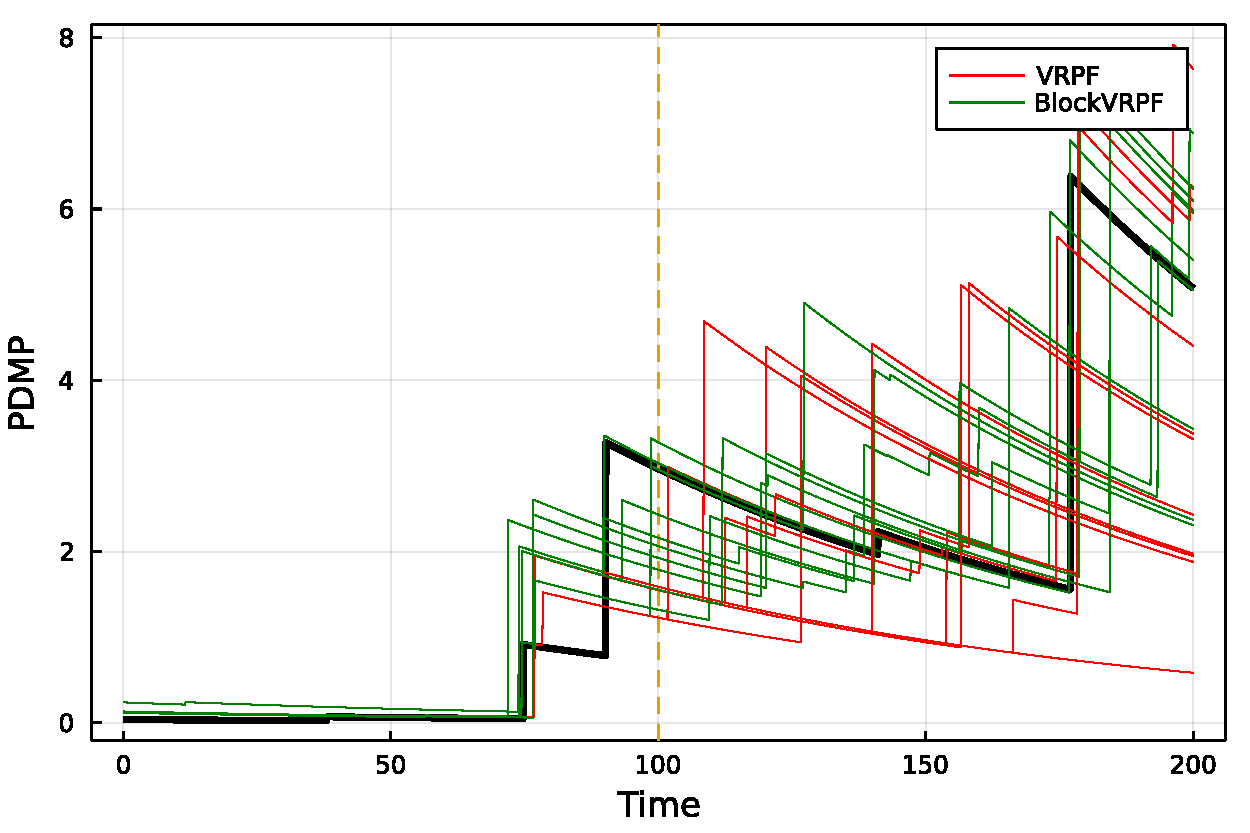
\includegraphics[width=\textwidth]{BlockVRPF_Illustration.pdf}
    \caption{Illustration of the correcting power of BlockVRPF sampler. Black line represents the actual PDMP we are interested. Given the same sampled jumps in the first block (time blocks are splitted by the yellow dashed line), both VRPF and BlockVPRF sampler were used to sample the jumps in the second block. These sampled processes are represented by red lines (VRPF) and green lines (BlockVRPF)}
    \label{BlockSMC_correction_illustration}
\end{figure}

\begin{algorithm}
    \caption{Block Variable Rate Particle Filter (BlockVRPF)}\label{Alg:BlockVRPF}
    \For{n=1}{
        \For{$i=1,2,...,N$}{
            Sample $X_1^{i}:=\left(k_1^i,\tau_{1,1:k_1^i}^i,\phi_{1,1:k_1^i}^i,\phi_0^i\right) \sim K_1(\cdot)$\;
            Set $Z_1^i:= X_1^i$ and $\mathcal{J}_1^i := \left(\tau_{1,1:k_1^i}^i,\phi_{1,1:k_1^i}^i\right)$\;
            Calculate the un-normalised weight 
            $$G_1\left(Z_1^i\right) := \frac{\gamma_1\left(Z_1^i\right)}{K_1\left(Z_1^i\right)}$$
        }
        \For {$i=1,2,...,N$}{
            Calculate the normalised weight $W_1^i$ such that 
            $$W_1^i \propto G_1(Z_1^i),\quad \sum_{i=1}^{N} W_1^i = 1$$
        }
    }
    \For {n = 2,3,...,P}{
        \For {i = 1,2,...,N}{
            Sample $A_{n-1}^i \sim \mathbf{r}\left(\cdot|\mathbf{W_{n-1}}\right)$\;
            Sample $M_{n-1}^i \sim K_{n,1}\left(\cdot|\mathcal{J}_{n-1}^{A_{n-1}^i}\right)$\;
            Sample $U_{n-1}^i:=\left(\mathring{\tau}_{n-1}^i,\mathring{\phi}_{n-1}^i\right) \sim K_{n,2}\left(\cdot|m_{n-1}^i,z_{1:n-1}^{A_{n-1}^{i}}\right)$\;
            Sample $X_n^i := \left(k_n^i,\tau_{n,1:k_n^i}^i,\phi_{n,1:k_n^i}^i\right) \sim K_{n,3}^1 \left(\cdot | m_{n-1}^i,u_{n-1}^i,z_{1:n-1}^{A_{N-1}^i}\right)K_{n,3}^2\left(\cdot|k_n^i,m_{n-1}^i,u_{n-1}^i,z_{1:n-1}^{A_{N-1}^i}\right)$\;
            Set $Z_n^i := \left(M_{n-1}^i,U_{n-1}^i,X_{n-1}^i\right)$ and $Z_{1:n}^i := \left(Z_{1:n-1}^{A_{n-1}^i},Z_n^i\right)$\;
            Define $\mathcal{J}_n^i$ according to \eqref{Iterative Jn:Case1}, \eqref{Iterative Jn:Case2} or \eqref{Iterative Jn:Case3} based on $\mathcal{J}_{n-1}^{A_{n-1}^i}$\;
            Calculate the incremental weight $G_n\left(z_{1:n}^i\right)$ according to \eqref{BlockVRPF_SMC_IncrementalWeight_Adjust_EmptyU}, \eqref{BlockVRPF_SMC_IncrementalWeight_Adjust_NonEmptyU} or \eqref{BlockVRPF_SMC_Incremental Weight_Birth}\;
        }
        \For {$n=1,...,N$}{
            Calculate the normalised weight $W_n^i$ such that 
            $$W_n^i \propto G_n(Z_{1:n}^i),\quad \sum_{i=1}^{N} W_n^i = 1$$
        }
    }
\end{algorithm}

\section{Static Parameter Estimations using Particle Gibbs}
In the previous section, we proposed a novel method that combines block sampling and VRPF to perform filtering on the piecewise deterministic Markov models, given the values of the static parameters in the model is known. In this section, we are trying to make inferences on these static parameters in the piecewise deterministic processes. 

There has been many Bayesian methods based around the SMC sampler proposed by various authors to estimate the static parameters of Markov models, such as Neal (2001) and Chopin (2002). More recently, Andrieu et al. (2010) and Chopin et al. (2013) showed that SMC methods can be combined with Markov Chain Monte Carlo (MCMC) methods to make estimations on the static parameters in state-space models. 
\subsection{Particle Markov Chain Monte Carlo (PMCMC) Methods }
The Particle Markov Chain Monte Carlo (PMCMC) is a class of Bayesian inference methods that combine SMC with MCMC to approximately generate samples from the posterior distribution of the parameters for models whose likelihood is intractable due to the presense of latent variables. Suppose the parameter $\theta \in \Theta$ of the model of interest has a prior density $\pi(\theta)$. Given observations $y_{1:T}$, we are interested in the posterior density $\pi_P(\theta|y_{1:P}) \propto \pi(\theta)p(y_{1:P}|\theta)$. When there are latent variables present in the model, the likelihood $p(y_{1:P}|\theta)$ will be given by 
\begin{equation}
    \label{PMCMC-marginal likelihood}
    p(y_{1:P}|\theta) = \int p(x_{1:P},y_{1:P}|\theta)dx_{1:P} = \int p(x_{1:P}|\theta) p(y_{1:P}|x_{1:P},\theta) dx_{1:P}
\end{equation}
which is intractable in most scenario. This hinders us from designing standard MCMC samplers targeting $p(\theta|y_{1:P})$. To alleviate this problem, one could include $x_{1:P}$ as auxiliary variables and target the extended density $\pi_P(\theta,x_{1:P}|y_{1:P})$ using a MCMC sampler. By targetting the extended density, we have an opportunity to implement a Gibbs sampler to sample from $\pi_P(\theta,x_{1:P}|y_{1:P})$ by the following scheme:
\begin{enumerate}[label=\textit{Step \arabic*.},leftmargin=*]
    \item Sample $\theta' \sim \pi_P(\theta|x_{1:P},y_{1:P})$
    \item Sample $x_{1:P} \sim \pi_P(x_{1:P}|\theta',y_{1:P})$
\end{enumerate}
Performing the sampling task in \textit{Step 1} is in general easy. If conjugate priors are used for $\theta$, one can sample exactly from the posterior density. As the unnomarlised density $\pi_P(\theta,x_{1:P},y_{1:P})$ can be evaluated point-wise, one can also replace \textit{Step 1} with a Matropolis-Hastings step when direct sampling is not possible. On the other hand, sampling from the denstiy in \textit{Step 2} is in general intractable except for some specific scenarios such as linear Gaussian models and finite state Hidden Markov models \citep{andrieu2010particle}. Hence, prcatically one should replace \textit{Step 2} with a Metropolis-Hastings update. In order ensure good performance of the MH update in \textit{Step 2}, ond should normally search for a "good" proposal distribution $q(x_{1:P})$ that is similar to $\pi_P(x_{1:P}|\theta',y_{1:P})$. As a result, a natural idea would be using the emprical distribution obtained by running an SMC algorithm targeting $\pi_P(x_{1:P}|\theta',y_{1:P})$ with $N$ particle as the proposal distribution for the MH update. From the previous chapter, we know that the SMC algorithm produces an approximation to its target density by
\begin{equation}
    \label{PMCMC - Approximation of Step 2 Distribution}
    \hat{\pi}_P(dx_{1:P}|\theta',y_{1:P}):=\sum_{n=1}^{N} W_P^n \delta_{x_{1:P}^n}(dx_{1:P})
\end{equation}
This gives us a way of designing a proposal distribution that is in fact an approximation of the actual density $\pi_P(x_{1:P}|\theta',y_{1:P})$. In fact, one can use the approximation defined in \eqref{PMCMC - Approximation of Step 2 Distribution} as the proposal distribution and this is the key idea behind the PMCMC methods. Sampling from $\hat{\pi}_P(dx_{1:P}|\theta',y_{1:P})$ is simple as one only needs the outputs from a single run of the corresponding SMC algorithm. However, the calculation of acceptance probability of the MH update requires one to compute the proposal density $q(dx_{1:P})$ that is in this case given by 
\begin{equation}
    q(x_{1:P}) := \mathbb{E}_{W_{1:P}^{1:N},x_{1:P}^{1:N}}\left[\hat{\pi}_P(dx_{1:P}|\theta',y_{1:P})\right]
\end{equation}
where the expectation is taken with respect to all the random variables generated by the SMC algorithm \citep{andrieu2010particle}. This is in general intractable, making the MH update in \textit{Step 2} impractical. One natural way to solve this problem would be using the 'auxiliary trick' again - to include all the random variables produced during the SMC algorithm as auxiliary variables and interpret the SMC algorihtm as a proposal kernel that generates a 'single sample' at each time. More specifically, let $\mathbf{X}_n := \left(X_n^1,X_n^2,...,X_n^N\right)$ and $\mathbf{A}_{n-1}:=\left(A_{n-1}^1,A_{n-1}^2,...,A_{n-1}^N\right)$ be the particles and ancestor indices generated at step $n$ of the SMC algorithm. Then, all the random variables generated during an SMC algorithm will be $\left(\mathbf{X}_1,...,\mathbf{X}_P,\mathbf{A}_1,...,\mathbf{A}_{P-1}\right)$ and the joint density of these random variables will be given by 
\begin{equation}
    \label{JointDensity-of-SMC}
    \begin{split}
        \psi_P^{N,\theta}(\textbf{x}_1,...,\textbf{x}_P,\textbf{a}_1,...,\textbf{a}_{P-1}) & := \left\{\prod_{j=1}^{N}K_1^{\theta}\left(x_1^j\right)\right\}\prod_{n=2}^{P}\left\{r^{\theta}\left(\textbf{a}_{n-1}|\textbf{W}_{n-1}\right)\prod_{j=1}^{N}K_n^{\theta}\left(x_n^j|x_{1:n-1}^{a_{n-1}^j}\right)\right\}
    \end{split}
\end{equation}
Such an SMC sampler will produce $N$ distinct paths, i.e. $X_{1:P}^1, X_{1:P}^2,...,X_{1:P}^N$. For a specific path, $X_{1:P}^k$, we can denote it as 
$$X_{1:P}^k : = X_{1:P}^{B_{1:P}^k}=\left(X_1^{B_1^k},X_2^{B_2^k},...,X_P^{B_P^k}\right)$$
with $B_P^k = k$ and $B_n^k = A_{n}^{B_{n+1}^k}$. To sample a single path from the proposal, one just need to sample the lineage index $k$ with probability $W_P^k$ and set $x_{1:P}^{'}:= x_{1:P}^{k}:=x_{1:P}^{b_{1:P}}$ with $b_P = k$. Since all the random variables from an SMC algorihtm are now included in the proposal distribution, we should also define a corresponding extended target distribution that includes $\theta$ and $\left(\mathbf{X}_1,...,\mathbf{X}_P,\mathbf{A}_1,...,\mathbf{A}_{P-1}\right)$. The design of the target distribution should fulfill the following two conditions:
\begin{enumerate}[label=\textit{Condition \arabic*.},leftmargin=*]
    \item The target distribution would still admit $\pi_P(\theta,x_{1:P}|y_{1:P})$ as a marginal.
    \item The target distribution should be as close as possible to the proposal distribution in a certain sense.
\end{enumerate}
The first condition needs to be fullfilled to ensure that we are still able to target the correct distribution as a marginal. We try to achieve the second condition in order to make sure that the MH update targeting this extended distribution is as efficient as possible. Inspired by this, we should consider factorising the extended target density in the form
\begin{equation}
    \label{PMCMC-Form of extended target}
    \tilde{\pi}_P(\theta,b_{1:P},\mathbf{x}_{1:P},\mathbf{a}_{1:P-1}) = \frac{\pi_{P}(\theta,x_{1:P}^{b_{1:P}},b_{1:P})}{N^P}\psi_P^{N,\theta}(\mathbf{x}_{1:P}^{-b_{1:P}},\mathbf{a}_{1:P-1}^{-b_{2:P}}|\theta,x_{1:P}^{b_{1:P}},b_{1:P})
\end{equation}  
where we define $\mathbf{x}_{1:P}^{-b_{1:P}} := \mathbf{x}_{1:P}\backslash x_{1:P}^{b_{1:P}}$ and similarly $\mathbf{a}_{1:P-1}^{-b_{2:P}} := \mathbf{a}_{1:P-1} \backslash a_{1:P-1}^{b_{2:P}}$. The first part of \eqref{PMCMC-Form of extended target} is included to meet the first condition. Practically, one could simply sample an lineage index $k$ with probability $W_P^k$ and set $b_P:=k$ and this would implicitly define the values of $b_{P-1},...,b_1$ through the relationship $b_n = a_n^{b_{n+1}}$. If the support of the proposal distributions used in the SMC algorithm, $K_1(dx_1)\prod_{j=2}^{P}K_j(dx_j|x_{1:j-1})$, encompasses that of $\pi_P$, the marginal density $\pi_P(\theta,x_{1:P}^{b_{1:P}},b_{1:P})/N^P$ would be the same as $\pi_P$, which is the actual density of our interest. 

The second part of \eqref{PMCMC-Form of extended target} is designed to meet the second requirement. As we need to define the distribution of the rest particles and ancestor indices and hope to design a distribution that are close to $\psi_P^{N,\theta}$. One way to do this is to define a conditional distribution of the rest particles and ancestor indices. Hence, we can define the joint distribution of $\textbf{X}_{1:P}^{-k}$ and $\textbf{A}_{1:P-1}^{-k}$ to be
\begin{equation}
    \label{Conditional SMC} 
    \begin{split}
        \psi_P^{N,\theta}\left(\mathbf{x}_{1:P}^{-b_{1:P}},\mathbf{a}_{1:P-1}^{-b_{2:P}}|x_{1:P}^{b_{1:P}},b_{1:P}\right) &:= \frac{\psi_P^{N,\theta}(\mathbf{x}_{1:P},\mathbf{a}_{1:P})}{K_1\left(x_1^{b_1}\right)\prod_{n=2}^P \left\{r\left(b_{n-1}|\mathbf{W}_{n-1}\right)K_n\left(x_n^{b_n}|x_{1:n-1}^{b_{1:n-1}}\right)\right\}}\\
        &= \left\{\prod_{1\leq j \leq N,j \neq b_1} K_1\left(x_1^j\right)\right\}\prod_{n=2}^P r\left(\mathbf{a}_{n-1}^{-b_{n}}|\mathbf{W}_{n-1},a_{n-1}^{b_n}\right) \\
        &\quad\quad\quad\quad \times \prod_{1 \leq j \leq N, j \neq b_n} K\left(x_n^j|x_{1:n-1}^{a_{n-1}^j}\right)
    \end{split}
\end{equation} 


Since Equation \eqref{Conditional SMC} is the conditional distribution of \(\left(\textbf{X}_{1:P}^{-b_{1:P}},\textbf{A}_{1:P-1}^{-b_{2:P}}\right)\) given the path \(\left(x_{1:P}^{b_{1:P}},b_{1:P}\right)\) in \(\tilde{\pi}_P^N\). This gives actaully inspires the idea of partible Gibbs sampler described in \cite{andrieu2010particle}. At each iteration, given we have obtained \(\left(\theta,b_{1:P},x_{1:P}^{b_{1:P}},\textbf{x}_{1:P}^{-b_{1:P}},\textbf{a}_{1:P-1}^{-b_{2:P}}\right)\), we can do the following to obtain a new set of random variables

\begin{enumerate}[label=\textit{Step \arabic*.},leftmargin=*]
    \item Sample $\theta^{*} \sim \tilde{\pi}_P^N\left(\theta|b_{1:P},x_{1:P}^{b_{1:P}},\textbf{x}_{1:P}^{-b_{1:P}},\textbf{a}_{1:P-1}^{-b_{2:P}}\right)$ 
    \item Sample $\textbf{X}_{1:P}^{*,-b_{1:P}},\textbf{A}_{1:P-1}^{*,-b_{2:P}} \sim \psi_P^{N,\theta^{*}}\left(\textbf{x}_{1:P}^{*,-b_{1:P}},\textbf{a}_{1:P-1}^{*,-b_{2:P}}|b_{1:P},x_{1:P}^{b_{1:P}}\right)$
    \item Sample $b_{1:P}^{*},x_{1:P}^{b_{1:P}^{*}} \sim \tilde{\pi}_P^N\left(b_{1:P}^{*},x_{1:P}^{b_{1:P}^{*}}|\theta^{*},\textbf{x}_{1:P}^{*,-b_{1:P}},\textbf{a}_{1:P-1}^{*,-b_{2:P}},b_{1:P},x_{1:P}^{b_{1:P}}\right)$
\end{enumerate}

As described in \cite{andrieu2010particle}, \textit{Step 1} of the above sampling scheme can be simplified to sampling $\theta^{*} \sim \pi_P(\theta^{*}|x_{1:P}^{b_{1:P}})$ and this still leaves the target density $\tilde{\pi}_P^N$ invariant. This is a special type of Gibbs sampler known as 'collapsed' Gibbs sampler which was discussed in \cite{liu2001monte} and \cite{van2008partially}. For complex models, directly sampling from \(\pi_P(\theta^{*}|x_{1:P}^{b_{1:P}})\) may not be possible either. In this case, one can insert a Metropolis-Hastings update to \textit{Step 1}. Given a transition kernel \(q(\,d\theta'|\theta)\), one can sample a candidate \(\theta'\) and set \(\theta^{*} := \theta'\) with probability 
\[
    \alpha(\theta,\theta') := 1 \wedge  \frac{\pi_P(\theta'|x_{1:P}^{b_{1:P}})q(\theta|\theta')}{\pi_P(\theta|x_{1:P}^{b_{1:P}})q(\theta'|\theta)} 
\]
Such a technique is termed as \textit{Metropolis-Hastings within Partially Collapsed Gibbs} (MHwPCG) and its correctness was described in \cite{van2008partially}. \textit{Step 2} of the scheme involves sampling from the conditional distribution defined by \(\psi_{P}^{N,\theta^{*}}\left(\mathbf{x}_{1:P}^{-b_{1:P}},\mathbf{a}_{1:P-1}^{-b_{2:P}}|x_{1:P}^{b_{1:P}},b_{1:P}\right)\). One can see that this conditional distribution only depends on the transition kernels $K_{1:P}$ and the resampling scheme $r$ used in the SMC algorithm. Hence, to sample from the conditional, one can employ an algorithm similar to the standard SMC algorithm, except for keeping a particular particle trajectory \(x_{1:P}^{b_{1:P}}\) fixed. Such an SMC sampler is termed as conditional SMC (cSMC) sampler and was first introduced in \cite{andrieu2010particle}. The details of the sampler is listed in Algorithm \ref{Alg:CSMC}.

\begin{algorithm}[htb!]
    \caption{Conditional SMC Sampler (cSMC)}\label{Alg:CSMC}
    Given a path $\left(X_{1:P}^{*},B_{1:P}\right)$\;
    \For{n=1}{
        \For {$j=1,2,3,...,N$}{
            \If{$j\neq B_1$}{
                Sample $X_{1}^j \sim K_1(\cdot)$\;
            }
            \If{$j=B_1$}{
                Set $X_1^j = X_1^{*}$\;
            }
            Calculate the weight $w_1^j$ and normalise the weights $W_1^j \propto w_1^j$\;
        }
    }
    \For{$n = 2,3,..,P$}{
        \For{$j=1,2,..,N$}{
            \If{$j \neq B_n$}{
                Sample $A_{n-1}^j \sim r\left(\cdot|\textbf{W}_{n-1}\right)$\;
                Sample $X_n^j \sim K_n\left(\cdot|X_{1:n-1}^{A_{n-1}^j}\right)$\;
            }
            \If{$j = B_n$}{
                Set $A_{n-1}^j = B_{n-1}$\;
                Set $X_n^j = X_n^{*}$\;
            }
            Calculate the weights $w_n^j$ and normalise them $W_{n}^j \propto w_n^j$\;
        }
    }
    
\end{algorithm}

Note that one could permute the indices of the particles in an SMC sampler while keeping the SMC sampler invariant. Hence, one could practically fix \(b_{1:P}\) to some convenient values (e.g \(b_i=1, i=1,2,..,P\)) to simplify the implementation of the cSMC sampler. 

\textit{Step 3} samples the ancestor indices \(b_{1:P}\)and the corresponding trajectory defined by the indices \(x_{1:P}^{b_{1:P}}\). Following \cite[Chapter~5]{lindsten2013backward}, the marginal is given by $\pi_P(\theta,x_{1:p}) \propto \pi(\theta)\pi^{\theta}_P(x_{1:P})$ and we can rewrite $\pi^{\theta}_P(x_{1:P})$ as 
\[
    \pi_{P}^{\theta}(x_{1:P}):= \pi_1^{\theta}(x_1) \prod_{n=2}^{P}\frac{\pi_n^{\theta}(x_{1:n})}{\pi_{n-1}^{\theta}(x_{1:n-1})} 
\]
Moreover, in an SMC sampler, the unnormalised weight \(w_n\) is given by 
\[
  w_n := \frac{\pi_n^{\theta}(x_{1:n})}{\pi_{n-1}^{\theta}(x_{1:n-1})K_n^{\theta}(x_n|x_{1:n-1})} 
\]
Hence, we have that 
\[
  \pi_P^{\theta}(x_{1:P}) := w_1K_1(x_1)\prod_{n=2}^{P} w_n K_n^{\theta}(x_n|x_{1:n-1})
\]
Hence, if we plugin \(x_{1:P}^{b_{1:P}}\), we would obtain 
\begin{equation}
    \label{PMCMC-another way of writing piP}
    \begin{split}
        \pi_P^{\theta}(x_{1:P}^{b_{1:P}}) &:= w_1^{b_1} K_1(x_1^{b_1})\prod_{n=2}^{P} w_n^{b_n} K_n^{\theta}(x_n^{b_n}|x_{1:n-1}^{b_{1:n-1}})\\
        &=\left\{\frac{w_1^{b_1}}{\sum_{i=1}^N w_1^i}K_1(x_1^{b_1})\prod_{n=2}^{P} \frac{w_n^{b_n}}{\sum_{i=1}^N w_n^i} K_n^{\theta}(x_n^{b_n}|x_{1:n-1}^{b_{1:n-1}})\right\}\left\{\prod_{n=1}^{P}\sum_{i=1}^N w_n^i\right\} \\
        &= W_P^{b_P}\left\{K_1(x_1^{b_1}) \prod_{n=2}^{P}W_{n-1}^{b_{n-1}}K_n(x_n^{b_n}|x_{1:n-1}^{b_{1:n-1}})\right\}\left\{\prod_{n=1}^{P}\sum_{i=1}^N w_n^i\right\} \\
        &=W_P^{b_P}\left\{K_1(x_1^{b_1}) \prod_{n=2}^{P}r(b_{n-1}|\mathbf{W}_{n-1})K_n(x_n^{b_n}|x_{1:n-1}^{b_{1:n-1}})\right\}\left\{\prod_{n=1}^{P}\sum_{i=1}^N w_n^i\right\}
    \end{split}
\end{equation}
If we substitute this into \eqref{PMCMC-Form of extended target}, we will obtain, after simplification 
\[
    \tilde{\pi}_P(\theta,b_{1:P},\mathbf{x}_{1:P},\mathbf{a}_{1:P-1}) = \frac{\pi(\theta)W_P^{b_P}}{N^P}\psi_P^{N,\theta}(\mathbf{x}_{1:P},\mathbf{a}_{1:P-1})\left\{\prod_{n=1}^{P}\sum_{i=1}^N w_n^i\right\}  \propto W_P^{b_P}
\]
Hence, we can see that to perform \textit{Step 3}, one simply choose \(b_P = k\) with probability \(W_P^k\) and set \(b_{n} := a_{n}^{b_{n+1}}\) for \(n=P-1,P-2,...,2,1\). The corresponding trajectory will then be obtained deterministically. These three steps completes one sweep of the particle Gibbs sampler and its full implementation is listed in Algorithm \ref{Alg: PG}.
\begin{algorithm}[htb!]
    \caption{particle Gibbs sampler}\label{Alg: PG}
        Initialise at any $X_{1:P}^{(0)}$,$k^{(0)}$ and $B_{1:P}^{(0)}$\;
        \For {$n=1,2,..$}{
            Sample $\theta^{(n)} \sim \pi_P\left(\cdot|x_{1:P}^{(n-1)}\right)$\;
            Sample $\textbf{X}_{1:P}^{(n),-k^{(n-1)}},\textbf{A}_{1:P-1}^{(n),-k^{(n-1)}} $ by running a cSMC sampler conditional on $X_{1:P}^{(n-1)}$ and $B_{1:P}^{(n-1)}$, outlined in Algorithm \ref{Alg:CSMC}\;
            Sample $k^{(n)} = j$ with probability $W_P^j$. Set $B_P^{(n)} = j$ and $B_m^{(n)} = A_{m}^{B_{m+1}^{(n)},k^{(n)}}$ for $m=P-1,..,2,1$\;
            Set $X_{1:P}^{(n)} = \left(X_{1}^{(n),B_{1}^{(n)}},...,X_P^{(n),B_{P}^{(n)}}\right)$\;
        } 
\end{algorithm}
\subsection{Particle Gibbs with Backward Sampling}\label{Section-BackwardSimulation}
We discussed the particle Gibbs sampler in the previous section. One of the major advantages of such type of sampler is that it does not rely on the asymptotics of \(N\) to be a valid MCMC sampler. However, the particle Gibbs sampler we discussed in the previous section is likelihood to have mixing issues. In the particle Gibbs sampler we discussed before, we only samples the ancestor index at $P$ according to the importance weight $\mathbf{W}_P$, and traces the ancestral lineage back of the particles to get a full path $X_{1:P}$ at each step. This may result in the particle Gibbs sampler having a poor mixing when there is significant degeneracy in the cSMC sampler. Such a problem is especially obvious when $P$ is large and $N$ is small since longer time and small number of particles often come with degeneracy. As the particle trajectory sampled in the previous iteration must be kept fixed in the cSMC algorithm, the next sampled particle trajectory would be therefore very similar to the previous one, resulting in a poor mixing of the Gibbs sampler. One way to solve this problem was proposed by \cite{whiteley2014backwardsampling} and further explored later by \cite{lindsten2012use}. The idea is to insert a backward simulation step to the particle Gibbs sampler to mitigate path degeneracy issues. In the context of particle Gibbs sampler, one can interpret this changing \textit{Step 3} of the particle Gibbs sweep to simulations of \(b_P,b_{P-1},..,b_1\). Hence, instead of performing the original \textit{Step 3}, we do the following
\begin{itemize}
    \item Sample \(b_P^{*} \sim \tilde{\pi}_P^{N}(b_P^{*}|\theta^{*},\textbf{x}_{1:P}^{*,-b_{1:P}},\textbf{a}_{1:P-1}^{*,-b_{2:P}},b_{1:P},x_{1:P}^{b_{1:P}})\)
    \item Sample \(b_{P-1}^{*} \sim \tilde{\pi}_P^{N}(b_{P-1}^{*}|\theta^{*},\textbf{x}_{1:P}^{*,-b_{1:P}},\textbf{a}_{1:P-1}^{*,-b_{2:P}},b_{1:P-1},x_{1:P-1}^{b_{1:P-1}},x_P^{b_P^{*}},b_{P}^{*})\)
    \item ......
    \item Sample \(b_{t}^{*} \sim \tilde{\pi}_P^{N}(b_{t}^{*}|\theta^{*},\textbf{x}_{1:P}^{*,-b_{1:P}},\textbf{a}_{1:P-1}^{*,-b_{2:P}},b_{1:t},x_{1:t}^{b_{1:t}},x_{t+1:P}^{b_{t+1:P}^{*}},b_{t+1:P}^{*})\)
    \item ......
    \item Sample \(b_{1}^{*} \sim \tilde{\pi}_P^{N}(b_{1}^{*}|\theta^{*},\textbf{x}_{1:P}^{*,-b_{1:P}},\textbf{a}_{1:P-1}^{*,-b_{2:P}},b_{1},x_{1}^{b_{1}},x_{2:P}^{b_{2:P}^{*}},b_{2:P}^{*})\)
\end{itemize}
Now, we are going to derive the conditional distribution of \(b_t^{*}\) listed above. One can see that the conditional distributions of $b_t^{*}$ is independent of \(\mathbf{x}_{t+1:P}^{-b_{t+1:P}^{*}}\) and \(\mathbf{a}_{t:P-1}^{-b_{t+1:P}^{*}}\). Therefore, by marginalising \(\psi_{P}^{N,\theta}\) over \(\mathbf{x}_{t+1:P}^{-b_{t+1:P}}\) and \(\mathbf{a}_{t:P-1}^{-b_{t+1:P}}\), we obtain 
\begin{equation}
    \label{PMCMC-Marginal of psi}
    \psi_{P}^{N,\theta}(\mathbf{x}_{1:t}^{-b_{1:t}},\mathbf{a}_{1:t-1}^{-b_{2:t}}|x_{1:P}^{b_{1:P}},b_{1:P}) := \prod_{\substack{j=1\\j \neq b_1}}^{N} K_1\left(x_1^j\right)\prod_{n=2}^t \left\{r\left(\mathbf{a}_{n-1}^{-b_{n}}|\mathbf{W}_{n-1},a_{n-1}^{b_n}\right)\prod_{\substack{j=1\\ j \neq b_n}}^{N} K_n(x_n^j|x_{1:n-1}^{a_{n-1}^j})\right\}
\end{equation}

Hence, the conditional distribution of $b_t^{*}$ will then be given by 
\begin{equation}
    \label{PMCMC-PGBS conditional}
    \begin{split}
        &\tilde{\pi}_P^{N}(b_t^{*}|\theta^{*},\textbf{x}_{1:t}^{*,-b_{1:t}},\textbf{a}_{1:t-1}^{*,-b_{2:t}},b_{1:t},x_{1:t}^{b_{1:t}},x_{t+1:P}^{b_{t+1:P}^{*}},b_{t+1:P}^{*}) \\\\
        &=\frac{\pi_P(\theta^{*},b_{1:t},b_{t+1:P}^{*},x_{1:t}^{b_{1:t}},x_{t+1:P}^{b_{t+1:P}^{*}})}{N^P}\psi_{P}^{N,\theta}(\mathbf{x}_{1:t}^{-b_{1:t}},\mathbf{a}_{1:t-1}^{-b_{2:t}}|b_{1:t},b_{t+1:P}^{*},x_{1:t}^{b_{1:t}},x_{t+1:P}^{b_{t+1:P}^{*}})\\\\
        &=\frac{\pi_P^{\theta^{*}}(x_{1:t}^{b_{1:t}},x_{t+1:P}^{b_{t+1:P}^{*}})}{\pi_t^{\theta^{*}}(x_{1:t}^{b_{1:t}})}\frac{\pi_t^{\theta^{*}}(x_{1:t}^{b_{1:t}})\pi(\theta^{*})}{N^P}\prod_{\substack{j=1\\j \neq b_1}}^{N} K_1\left(x_1^j\right)\prod_{n=2}^t \left\{r\left(\mathbf{a}_{n-1}^{-b_{n}}|\mathbf{W}_{n-1},a_{n-1}^{b_n}\right)\prod_{\substack{j=1\\ j \neq b_n}}^{N} K_n(x_n^j|x_{1:n-1}^{a_{n-1}^j})\right\}\\\\
        &=\frac{\pi_P^{\theta^{*}}(x_{1:t}^{b_{1:t}},x_{t+1:P}^{b_{t+1:P}^{*}})}{\pi_t^{\theta^{*}}(x_{1:t}^{b_{1:t}})}\frac{\pi(\theta^{*})W_t^{b_t}}{N^P}\psi_t^{N,\theta^{*}}(\mathbf{x}_{1:t},\mathbf{a}_{1:t-1})\left\{\prod_{n=1}^{t}\sum_{i=1}^N w_n^i\right\} \propto W_t^{b_t} \frac{\pi_P^{\theta^{*}}(x_{1:t}^{b_{1:t}},x_{t+1:P}^{b_{t+1:P}^{*}})}{\pi_t^{\theta^{*}}(x_{1:t}^{b_{1:t}})}
    \end{split} 
\end{equation}
where the last line is derived in a similar way as we did in \eqref{PMCMC-another way of writing piP}. In fact, the backward sampling step inserted in the particle Gibbs corresponds to the backward smoothing schedule of a standard SMC algorithm. We summarise the corresponding particle Gibbs with backward sampling (PGBS) sampler in Algorithm \ref{Alg: PGBSi}

\begin{algorithm}[htb!]
    \caption{particle Gibbs with Backward Simulation}\label{Alg: PGBSi}
    Start at $\theta^{(0)}$, $X_{1:P}^{(0)}$ and $B_{1:P}^{(0)}$ arbitrarily\;
    \For{n=1,2,...}{
        Sample $\theta^{(n)} \sim \pi_{P}\left(\cdot|X_{1:P}^{(n-1)}\right)$ using e.g. a MH kernel\;
        Run a cSMC algorithm conditional on $x_{1:P}^{(n-1)}, b_{1:P}^{(n-1)}$ and $\theta^{(n)}$, outlined in Algorithm \ref{Alg:CSMC}, to get $\textbf{X}_{1:P}^{(n)}$ and $\textbf{A}_{1:P-1}^{(n)}$ and $\mathbf{W}_{1:P}^{(n)}$\;
        \For{$t=P,P-1,...,2,1$}{
            Set $b_t^{(n)}=k$ with probability 
            \[
                W_t^{(n),k}\frac{\pi_P^{\theta^{(n)}}(x_{1:t}^{(n),k},x_{t+1:P}^{(n),b_{t+1:P}^{*}})}{\pi_t^{\theta^{*}}(x_{1:t}^{(n),k})}
            \]
            where $b_t=k$ and $b_{j} = a_{j}^{(n),b_{j+1}}$
        }
        Set \(x_{1:P}^{(n)}:= x_{1:P}^{(n),b_{1:P}^{(n)}}\)
    }
\end{algorithm}
The PGBS sampler generally has much better than the standard particle Gibbs sampler. Due to the addition of the backward sampling step, we would be able to explore all the possible trajectories created by the combinations of particles obtained from the cSMC algorithm. As a result, the new sampled trajectory would be highly likely significantly different from the previous one. This brings a big improvement on the mixing in the state space, hence the particle Gibbs sampler overall. 

For the VRPF method, denote \(\check{\mathcal{J}}_{n}:=(\check{k}_n,\check{\tau}_{n,1:\check{k}_n},\check{\phi}_{n,1:\check{k}_n})\) be the collection of jump times and values that define the PDP in the interval \((t_{n-1},t_P)\), we then should have that 
\begin{equation*}
    \check{k}_n := \sum_{j=n}^{P} k_j \quad\quad\quad \check{\tau}_{n,1:\check{k}_n} :=  \bigcup_{j=n}^{P} \left\{\tau_{j,1:k_j}\right\} \quad\quad\quad \check{\phi}_{n,1:\check{k}_n} :=  \bigcup_{j=n}^{P} \left\{\phi_{j,1:k_j}\right\}
\end{equation*}
Suppose the ancestor indices $b_{n+1}^{*},..,b_P^{*}$ have already been sampled and the corresponding particles \(x_{n}^{b_n^*},...,x_P^{b_P^*}\) form $\check{\mathcal{J}}_{n+1}^{*}$. If $\check{k}_{n+1}^{*}>0$, the unnormalised backward sampling incremental weight will be given by 
\begin{equation}
    \label{PMCMC - VRPF Backward Simulation Weight 1}
    \mathcal{G}_{n|P}(x_{1:n}^{b_{1:n}}) := \frac{f(\check{\tau}_{n+1,1}^{*}|\hat{\tau}_{n,\hat{k}_n})g(\check{\phi}_{n+1,1}^{*}|\hat{\phi}_{n,\hat{k}_n},\hat{\tau}_{n,\hat{k}_n},\check{\tau}_{n+1,1}^{*})p(y_{(t_n,\check{\tau}_{n+1,1}^{*}]}|\hat{\phi}_{n,\hat{k}_n})}{S(\hat{\tau}_{n,\hat{k}_n},t_n)}
\end{equation}
If $\check{k}_{n+1}^{*} = 0$, the corresponding backward sampling incremental weight will be given by 
\begin{equation}
    \label{PMCMC - VRPF Backward Simulation Weight 2}
    \mathcal{G}_{n|P}(x_{1:n}^{b_{1:n}}) = \frac{S(\hat{\tau}_{n,\hat{k}_n},t_P)p(y_{(t_n,t_P]}|\hat{\phi}_{n,\hat{k}_n})}{S(\hat{\tau}_{n,\hat{k}_n},t_n)}
\end{equation}

For the BlockVRPF sampler, we use the same notation $\check{\mathcal{J}}_{n}$ to denote the collection of jump times and values defined by \(Z_{n},..,Z_p\). Given $Z_{n+1}^{b_{n+1}^{*}},..,Z_{P}^{b_{P}^{*}}$ and the corresponding $\check{\mathcal{J}}_{n}^{*}$, if $M_{n}^{*} = 1$, the corresponding backward sampling incremental weight would be given by 
\begin{equation}
    \label{PMCMC - BlockVRPF Backward Simulation Weight 1}
    \mathcal{G}_{n|P}(z_{1:n}^{b_{1:n}}) := \frac{\mathbbm{I}(\mathring{\tau}_n^{*}>\hat{\tau}_{n,\hat{k}_n})f(\mathring{\tau}_n^{*}|\hat{\tau}_{n,\hat{k}_n})g(\mathring{\phi}_n^P{*}|\hat{\phi}_{n,\hat{k}_n},\mathring{\tau}_n^{*},\hat{\tau}_{n,\hat{k}_n})\mu(M_n^{*}|z_{1:n},z_{n+1:P}^{b_{n+1:P}^*})}{S(\hat{\tau}_{n,\hat{k}_n},t_n)p(y_{(\mathring{\tau}_n^{*},t_n]}|\hat{\phi}_{n,\hat{k}_n})}
\end{equation}
When $M_n^{*} = 0$ and $U_n^{*} = \emptyset$, if $\check{k}_n = 0$, we have 
\begin{equation}
    \label{PMCMC - BlockVRPF Backward Simulation Weight 2}
    \mathcal{G}_{n|P}(z_{1:n}^{b_{1:n}}) := \frac{\mathbbm{I}(\hat{\tau}_{n,\hat{k}_n} < t_{n-1})S(\hat{\tau}_{n,\hat{k}_n},t_P)\mu(M_n^{*}|z_{1:n},z_{n+1:P}^{b_{n+1:P}^*})p(y_{(t_n,t_P]}|\hat{\phi}_{n,\hat{k}_n})}{S(\hat{\tau}_{n,\hat{k}_n},t_n)}
\end{equation}
If $\check{k}_n^{*} > 0$, we then have 
\begin{multline}
    \label{PMCMC - BlockVRPF Backward Simulation Weight 3}
    \mathcal{G}_{n|P}(z_{1:n}^{b_{1:n}}) := \frac{f(\check{\tau}_{n+1,1}^{*}|\hat{\tau}_{n,\hat{k}_n})g(\check{\phi}_{n+1,1}^{*}|\hat{\phi}_{n,\hat{k}_n},\hat{\tau}_{n,\hat{k}_n},\check{\tau}_{n+1,1}^{*})p(y_{(t_n,\check{\tau}_{n+1,1}^{*}]}|\hat{\phi}_{n,\hat{k}_n})}{S(\hat{\tau}_{n,\hat{k}_n},t_n)} \\
    \times \mathbbm{I}(\hat{\tau}_{n,\hat{k}_n} < t_{n-1})\mu(M_n^{*}|z_{1:n},z_{n+1:P}^{b_{n+1:P}^*})
\end{multline}
In the case \(U_n^{*} \neq \emptyset\), we should have 
\begin{multline}
    \label{PMCMC - BlockVRPF Backward Simulation Weight 4}
    \mathcal{G}_{n|P}(z_{1:n}^{b_{1:n}}) := \frac{f(\mathring{\tau}_n^{*}|\hat{\tau}_{n,\hat{k}_n-1})g(\mathring{\phi}_n^{*}|\hat{\phi}_{n,\hat{k}_{n}-1},\hat{\tau}_{n,\hat{k}_n-1},\mathring{\tau}_n^{*})}{f(\hat{\tau}_{n,\hat{k}_{n}}|\hat{\tau}_{n,\hat{k}_n-1})g(\hat{\phi}_{n,\hat{k}_{n}}|\hat{\phi}_{n,\hat{k}_{n}-1},\hat{\tau}_{n,\hat{k}_n-1},\mathring{\tau}_n^{*})}
    \times\frac{p(y_{(\hat{\tau}_{n,\hat{k}_n}\wedge \mathring{\tau}_n^{*},\mathring{\tau}_n^{*})}|\hat{\phi}_{n,\hat{k}_n-1})}{p(y_{(\hat{\tau}_{n,\hat{k}_n}\wedge \mathring{\tau}_n^{*},t_n)}|\hat{\phi}_{n,\hat{k}_n-1},\hat{\phi}_{n,\hat{k}_n})}\\\\
    \times \frac{\mu(M_n^{*}|z_{1:n},z_{n+1:P}^{b_{n+1:P}^*})\lambda(\hat{\tau}_{n,\hat{k}_{n}},\hat{\phi}_{n,\hat{k}_{n}}|z_{1:n},z_{n+1:P}^{b_{n+1:P}^*})}{S(\hat{\tau}_{n,\hat{k}_{n}},t_n)}\times\mathbbm{I}(\hat{\tau}_{n,\hat{k}_n}>t_{n-1},\mathring{\tau}_{n}^{*}>\hat{\tau}_{n,\hat{k}_n-1})
\end{multline}
\section{Auxiliary Variable Rejuvenation}
In this section, we discussed the rejuvenation step introduced by \cite{finke2014static} to improve the mixing of the particle Gibbs scheme. For the BlockVRPF scheme, the incremental weights at step $n$, described in Equation \eqref{BlockVRPF_SMC_IncrementalWeight_Adjust_EmptyU},\eqref{BlockVRPF_SMC_IncrementalWeight_Adjust_NonEmptyU} and \eqref{BlockVRPF_SMC_Incremental Weight_Birth}, involve a likelihood ratio of the observations given the original PDP and the modified PDP. Hence, if a modification (i.e. a birth move or a birth move) on a particular particle moves the PDP from a wrong position to the correct position, the likelihood ratio will become so large that this specific particle will be dominating over all the others. In this case, the particle Gibbs sampler will be stuck in this specific path and it will be very hard for a new path to be proposed, even though it is not a path that fits the observations well. 

The rejuvenation step proposed by \cite{finke2014static} can be used to solve this problem. This step is suitable whenever the SMC filtering scheme involves auxiliary variables. In the BlockVRPF scheme, what we are really interested is the distribution of variables $(x_{1,m},x_{2,m},..,x_{n-1,m},x_n)$ and $\Theta$. Therefore, we are only interested in the distribution $\gamma_{n}(x_{1,m},..,\allowbreak x_{n-1,m},x_n)$ in Equation \eqref{Block-VRPF Target}. Hence, $M_{1:n-1}$ and $U_1^{'},...,U_{n-1}^{'}$ are the auxiliary variables appeared in the target. In the standard particle Gibbs scheme, we propose a new value of $\Theta$ conditioning on both the interested and auxiliary variables. The rejuvenation step, instead, samples $\Theta$ conditioning on the interested variables only. Then, all the auxiliary variables will be re-sampled conditioning on the interested variable. Hence, if the sampled path $X_{1:P}$ can be splitted into the interested variables $X_I$ and auxiliary variables $X_A$ (i.e. $X_{1:P} := (X_I,X_A)$) and the target density $\pi_{P}(\theta,x_{1:P}) := \Tilde{\pi}_P(\theta,x_I)\times L(x_A|x_I)$, we will split the first step at each particle Gibbs sweep. This method will be outlined in Algorithm \ref{particle Gibbs-rejuvenation}

\begin{algorithm}[htb!]
    \caption{particle Gibbs with rejuvenation step}
            Initialise $\theta^{(0)}$, $X_{1:P}^{(0)}$ and $B_{1:P}^{(0)}$ arbitrarily\;
            \For {n=1,2,...}{
                Sample $\theta^{(n)} \sim \Tilde{\pi}_{P}\left(\cdot|x_I^{(n-1)}\right)$\;
                Sample $x_A^{*} \sim L\left(\cdot|x_I^{(n-1)}\right)$\;
                Set $X_{1:P}^{(n-1)} := \left(x_I^{(n-1)},x_A^{*}\right)$\;
                Run a cSMC algorithm conditional on $X_{1:P}^{(n-1)}, B_{1:P}^{(n-1)}$, outlined in Algorithm \ref{Alg:CSMC}, to get $\textbf{X}_{1:P}^{(n)}$ and $\textbf{A}_{1:P-1}^{(n)}$\;
                Run a backward simulation to get $B_{1:P}^{(n)}$ using the same method as in Algorithm \ref{Alg: PGBSi}\;
                Set $X_{1:P}^{(n)} = \left(X_1^{(n),B_{1}^{(n)}},...,X_P^{(n),B_{P}^{(n)}}\right)$\;
            }
    \label{particle Gibbs-rejuvenation}
\end{algorithm}

Note that the rejuvenation step re-samples the auxiliary variables, which are the modification moves as well as the jump times and values being modified at each SMC step. Hence, this gives the path a chance to have another modification move or another jump times and values to be modified. As such, the likelihood ratio of this specific particle will possibly be decreased, giving other particles from the SMC step an opportunity to be chosen at each sweep. Therefore, such a rejuvenation step will help the particle Gibbs scheme to escape from the stuck path, hence improving the mixing of the chain. 
\newpage
\bibliographystyle{icml2020}
\bibliography{reference}
\end{document}
